\chapter{Monte Carlo Synthetic Acceleration\\ Methods for the $SP_N$ Equations}
\label{ch:spn_equations}

In this chapter, we briefly derive the simplified $P_N$ ($SP_N$)
equations, closely following the work of Evans
\cite{evans_simplified_2013}, in order to gain full understanding of
the underlying system and its potential behavior in a Monte Carlo
context. From the $P_N$ equations, we apply a set of approximations to
yield the $SP_N$ equations for fixed source and criticality
problems. Using the fully-formed linear operator for the transport
problem, we explore solutions to the $SP_N$ equations with Monte Carlo
Synthetic Acceleration using a challenging light water reactor fuel
assembly criticality calculation as the driving problem. Several
difficulties arise when applying MCSA to these problems that were not
observed when investigating the simple transport system in the
previous chapter.

For Jacobi-based preconditioners, convergence with MCSA is difficult
if not impossible for ill-conditioned systems with this behavior
demonstrated using a simple neutron diffusion problem. In order to
effectively solve the $SP_N$ equations for the fuel assembly problem,
a suite of preconditioners along with a relaxation scheme is developed
and studied within the context of MCSA. Using these preconditioners,
several additional issues are observed and alleviated to a certain
extent by applying the reduced domain approximation. MCSA solutions
for the fuel assembly problem are then verified by comparing the
solutions against production Krylov solvers for problems with varying
numbers of energy groups. Finally performance is analyzed through
comparison with those same Krylov solvers in terms of both iterative
performance and CPU timing using the same set of problems utilized for
the verification.

%%---------------------------------------------------------------------------%%
\section{The Neutron Transport Equation}
\label{sec:transport_eq}
As a starting point for the $SP_N$ equations we define the
time-independent neutron transport equation
\cite{lewis_computational_1993}:
\begin{multline}
  \hat{\Omega} \cdot \vec{\nabla} \psi(\vec{r},\hat{\Omega},E) +
  \sigma(\vec{r},E) \psi(\vec{r},\hat{\Omega},E) = \\ \iint
  \sigma_s(\vec{r},E' \rightarrow E,\hat{\Omega}' \cdot \hat{\Omega})
  \psi(\vec{r},\hat{\Omega}',E') d\Omega' dE' +
  q(\vec{r},\hat{\Omega},E)\:,
  \label{eq:general_transport}
\end{multline}
with the variables defined as:
\begin{itemize}
\item $\vec{r}$ - neutron spatial position
\item $\hat{\Omega}$ - neutron streaming direction with radial
  component $\mu$ and azimuthal component $\omega$
\item $\hat{\Omega}' \cdot \hat{\Omega} = \mu_0$ is the angle of
  scattering
\item $E$ - neutron energy
\item $\psi(\vec{r},\hat{\Omega},E)$ - angular flux
\item $\sigma(\vec{r},E)$ - total interaction cross section
\item $\sigma_s(\vec{r},E' \rightarrow E,\hat{\Omega}')$ - probability
  of scattering from direction $\hat{\Omega}'$ into an angular domain
  $d\hat{\Omega}'$ about the direction $\hat{\Omega}$ and from energy
  $E'$ to an energy domain $dE'$ about energy $E$
\item $q(\vec{r},\hat{\Omega},E)$ - external source of neutrons.
\end{itemize}
For this work, it is sufficient to formulate
Eq~(\ref{eq:general_transport}) in 1-dimensional Cartesian geometry:
\begin{multline}
  \mu \frac{\partial}{\partial x} \psi(x,\mu,E) + \sigma(x,E)
  \psi(x,\mu,E) = \\ \iint \sigma_s(x,E' \rightarrow E,\hat{\Omega}'
  \cdot \hat{\Omega}) \psi(x,\hat{\Omega}',E') d\Omega' dE' +
  \frac{q(x,E)}{4 \pi}\:,
  \label{eq:cart_1d_transport}
\end{multline}
where the angular component of the solution is no longer dependent on
the azimuthal direction of travel and an isotropic source of neutrons
is assumed. In addition, for fission systems the eigenvalue form of
the transport equation is:
\begin{multline}
  \hat{\Omega} \cdot \vec{\nabla} \psi(\vec{r},\hat{\Omega},E) +
  \sigma(\vec{r},E) \psi(\vec{r},\hat{\Omega},E) = \\ \iint
  \sigma_s(\vec{r},E' \rightarrow E,\hat{\Omega}' \cdot \hat{\Omega})
  \psi(\vec{r},\hat{\Omega}',E') d\Omega' dE' + \\ \frac{1}{k} \chi(E)
  \iint \nu \sigma_f(\hat{r},E') \psi(\vec{r},\hat{\Omega}',E')
  d\Omega' dE' + q(\vec{r},\hat{\Omega},E) \:,
  \label{eq:eigenvalue_transport}
\end{multline}
with the additional variables defined as
\begin{itemize}
\item $k$ - multiplication factor
\item $\chi(E)$ - fission neutron energy spectrum
\item $\nu$ - average number of neutrons per fission
\item $\sigma_f(r,E')$ - fission cross section\:.
\end{itemize}
In 1-dimensional Cartesian geometry,
Eq~(\ref{eq:eigenvalue_transport}) becomes:
\begin{multline}
  \mu \frac{\partial}{\partial x} \psi(x,\mu,E) + \sigma(x,E)
  \psi(x,\mu,E) = \\ \iint \sigma_s(x,E' \rightarrow
  E,\hat{\Omega}' \cdot \hat{\Omega}) \psi(x,\hat{\Omega}',E')
  d\Omega' dE' + \\ \frac{1}{k} \chi(E)
  \iint \nu \sigma_f(x,E') \psi(x,\hat{\Omega}',E') d\Omega'
  dE' + \frac{q(x,E)}{4 \pi}\:.
  \label{eq:cart_1d_eigenvalue}
\end{multline}

%%---------------------------------------------------------------------------%%
\section{Derivation of the Monoenergetic $SP_N$ Equations}
\label{sec:spn_equations}
The $P_N$ equations as derived in \cite{lewis_computational_1993}
give $N+1$ coupled first-order equations capturing the spatial and
angular-dependence of the solution:
\begin{equation}
   \frac{1}{2n+1} \frac{\partial}{\partial x}\Big[ (n+1) \phi_{n+1} + n
     \phi_{n-1} \Big] + \Sigma_n \phi_n = q\delta_{n0} \:,
  \label{eq:final_pn_equations}
\end{equation}
where $\Sigma_n = \sigma-\sigma_{sn}$ and the summations are truncated
at some level of approximation $N$ such that $n = 0,1,\dotsc,N$. This
yields a set of $N+1$ equations for $N+2$ flux moments. In multiple
dimensions, the equation set becomes large and coupled not only
through angular moments but also through the spatial variables. As a
simpler alternative to multidimensional $P_N$ solutions, Gelbard
recognized in 1960 that the planar $P_N$ equations could be simplified
and applied an ad-hoc method to extend them to multiple dimensions,
yielding the $SP_N$ equations. These equations are not only fewer in
number, but also take on a diffusion-like form while maintaining the
angular character of the flux, making them amenable to solutions with
modern diffusion methods.

First, the $P_N$ equations can be simplified to $(N+1)/2$ second-order
equations by solving for the $n^{th}$ Legendre flux moment in the
odd-order equations:
\begin{equation}
  \phi_n = \frac{1}{\Sigma_n}\Bigg[ q \delta_{no} -
    \frac{\partial}{\partial x}\Big(\frac{n}{2n+1}\phi_{n-1} +
    \frac{n+1}{2n+1} \phi_{n+1} \Big) \Bigg]\:, 
  \label{eq:odd_moments}
\end{equation}
for $n = 1,3,\cdots,N$ and $\delta_{no} = 0\ \forall n \neq 0$. We can
insert the odd moments into Eq~(\ref{eq:final_pn_equations}) to get a
reduced group of equations for the even moments:
\begin{multline}
  -\frac{\partial}{\partial x}
  \Bigg[\frac{n}{2n+1}\frac{1}{\Sigma_{n-1}} \frac{\partial}{\partial
      x} \Big(\frac{n-1}{2n-1} \phi_{n-2} + \frac{n}{2n-1}\phi_n \Big)
    \\+ \frac{n+1}{2n+1}\frac{1}{\Sigma_{n+1}} \frac{\partial}{\partial
      x} \Big(\frac{n+1}{2n+3}\phi_n + \frac{n+2}{2n+3}\phi_{n+2}\Big)
    \Bigg] \\+ \Sigma_n \phi_n = q \delta_{n0}\ \ \ \ \ \ \ \ \ n =
  0,2,4,\cdots,N\:.
  \label{eq:reduced_pn}
\end{multline}
Immediately, we note the diffusion-like nature of
Eq~(\ref{eq:reduced_pn}) as compared to the original $P_N$
equations. To extend these equations to multiple dimensions, Gelbard
simply replaced the planar spatial derivatives in the reduced set of
equations with general multidimensional gradient operators:
\begin{multline}
  -\nabla \cdot \Bigg[\frac{n}{2n+1}\frac{1}{\Sigma_{n-1}} \nabla
    \Big(\frac{n-1}{2n-1} \phi_{n-2} + \frac{n}{2n-1}\phi_n \Big) \\+
    \frac{n+1}{2n+1}\frac{1}{\Sigma_{n+1}} \nabla
    \Big(\frac{n+1}{2n+3}\phi_n + \frac{n+2}{2n+3}\phi_{n+2}\Big)
    \Bigg] \\+ \Sigma_n \phi_n = q \delta_{n0}\ \ \ \ \ \ \ \ \ n =
  0,2,4,\cdots,N\:,
  \label{eq:spn_equations}
\end{multline}
yielding a multidimensional set of $(N+1)/2$ angular coupled equations
defined as the $SP_N$ equations. As with the $P_N$ equations, we
provide closure to this set of equations with $\phi_{N+1} = 0$. As a
concrete example, we will consider the $SP_7$ equations:
\begin{subequations}
  \begin{gather}
    -\nabla \cdot \frac{1}{3 \Sigma_1} \nabla ( \phi_0 + 2\phi_2 ) +
    \Sigma_0 \phi_0 = q \\ 
    -\nabla \cdot \Bigg[ \frac{2}{15 \Sigma_1} \nabla ( \phi_0 + 2\phi_2
      ) + \frac{3}{35 \Sigma_3}\nabla( 3\phi_2 + 4\phi_4)\Bigg] +
    \Sigma_2 \phi_2 = 0\\
    -\nabla \cdot \Bigg[ \frac{4}{63 \Sigma_3} \nabla ( 3\phi_2 +
      4\phi_4 ) + \frac{5}{99 \Sigma_5}\nabla( 5\phi_4 +
      6\phi_6)\Bigg] + \Sigma_4 \phi_4 = 0\\
    -\nabla \cdot \Bigg[ \frac{6}{143 \Sigma_5} \nabla ( 5\phi_4 +
      6\phi_6 ) + \frac{7}{195 \Sigma_7}\nabla(7\phi_6)\Bigg] +
    \Sigma_6 \phi_6 = 0 \:.
  \end{gather}
  \label{eq:sp7_equations}
\end{subequations}
To further modify these equations, we can use a change of variables to
create a new group of equations such that the gradients are operating
on a single vector:
\begin{subequations}
  \begin{gather}
    u_1 = \phi_0 + 2\phi_2 \\
    u_2 = 3\phi_2 + 4\phi_4 \\
    u_3 = 5\phi_4 + 6\phi_6 \\
    u_4 = 7\phi_6 \:.
  \end{gather}
  \label{eq:spn7_subs}
\end{subequations}
When substituted into Eq~(\ref{eq:sp7_equations}), these terms give:
\begin{subequations}
  \begin{gather}
    -\nabla \cdot \frac{1}{3 \Sigma_1} \nabla u_1 + \Sigma_0 \Bigg[
    u_1 - \frac{2}{3}u_2 + \frac{8}{15}u_3 - \frac{16}{35}u_4 \Bigg]
    = -q \\
    -\nabla \cdot \Bigg[ \frac{2}{15 \Sigma_1} \nabla u_1 +
    \frac{3}{35 \Sigma_3} \nabla u_2 \Bigg] + \Sigma_2 \Bigg[
    \frac{1}{3}u_2 - \frac{4}{15}u_3 + \frac{8}{35}u_4 \Bigg] = 0 \\
    -\nabla \cdot \Bigg[ \frac{4}{63 \Sigma_3} \nabla u_2 +
    \frac{5}{99 \Sigma_5} \nabla u_3 \Bigg] + \Sigma_4 \Bigg[
    \frac{1}{5}u_3 - \frac{6}{35}u_4 \Bigg] = 0 \\ 
    -\nabla \cdot \Bigg[ \frac{6}{143 \Sigma_5} \nabla u_3 +
    \frac{7}{195 \Sigma_7} \nabla u_4 \Bigg] + \Sigma_6 \Bigg[
    \frac{1}{7}u_4 \Bigg] = 0 \:.
  \end{gather}
  \label{eq:spn7_subs_equations}
\end{subequations}
If we rearrange Eq~(\ref{eq:spn7_subs_equations}) such that only one
divergence operation is present in each equation, we can formulate
this as a matrix system of 4 equations in the case of the $SP_7$
approximation:
\begin{equation}
  -\nabla \cdot D_n \nabla u_n + \sum_{m=1}^4 A_{nm} u_m =
  q_n\ \ \ \ \ \ \ n = 1,2,3,4\:,
  \label{eq:spn_matrix}
\end{equation}
with $\mathbf{u}$ the vector of solution variables:
\begin{equation}
  \mathbf{u} = ( u_1\ \ u_2\ \ u_3\ \ u_4 )^T \:,
  \label{eq:spn7_solution_vector}
\end{equation}
$\mathbf{D}$ the vector of effective diffusion coefficients:
\begin{equation}
  \mathbf{D} = \Bigg( \frac{1}{3\Sigma_1}\ \ \frac{1}{7\Sigma_3}\ \
  \frac{1}{11\Sigma_5}\ \ \frac{1}{15\Sigma_7} \Bigg)^T\:,
  \label{eq:spn7_diffusion_coeffs}
\end{equation}
$\mathbf{q}$ the vector of source terms where the $0^{th}$ moment
source has now been distributed through the system:
\begin{equation}
  \mathbf{q} = (
  q\ \ -\frac{2}{3}q\ \ \frac{8}{15}q\ \ -\frac{16}{35}q )^T\:,
  \label{eq:spn7_source_vector}
\end{equation}
and $\mathbf{A}$ a matrix of angular scattering terms:
% NOTE: I copied the following matrix directly out of Tom's tech note
% on the SPn equations which I am effectively following here because I
% was feeling lazy. I have verified its correctness.
\begin{equation}
  \mathbf{A} = 
  {\tiny \begin{bmatrix}
    (\Sigma_0) &
    (-\frac{2}{3}\Sigma_0) &
    (\frac{8}{15}\Sigma_0) &
    (-\frac{16}{35}\Sigma_0) \\
    %%
    &&&\\
    %%
    (-\frac{2}{3}\Sigma_0) &
    (\frac{4}{9}\Sigma_0 + \frac{5}{9}\Sigma_2) &
    (-\frac{16}{45}\Sigma_0 - \frac{4}{9}\Sigma_2) &
    (\frac{32}{105}\Sigma_0 + \frac{8}{21}\Sigma_2) \\
    %%
    &&&\\
    %%
    (\frac{8}{15}\Sigma_0) &
    (-\frac{16}{45}\Sigma_0 - \frac{4}{9}\Sigma_2) &
    (\frac{64}{225}\Sigma_0 + \frac{16}{45}\Sigma_2 + \frac{9}{25}\Sigma_4) &
    (-\frac{128}{525}\Sigma_0 - \frac{32}{105}\Sigma_2 - \frac{54}{175}\Sigma_4)
    \\ 
    %%
    &&&\\
    %%
    (-\frac{16}{35}\Sigma_0) &
    (\frac{32}{105}\Sigma_0 + \frac{8}{21}\Sigma_2) &
    (-\frac{128}{525}\Sigma_0 - \frac{32}{105}\Sigma_2 - \frac{54}{175}\Sigma_4)
    & 
    (\frac{256}{1225}\Sigma_0 + \frac{64}{245}\Sigma_2 +
    \frac{324}{1225}\Sigma_4 + \frac{13}{49}\Sigma_6)
  \end{bmatrix}}\:.
  \label{eq:A_matrix}
\end{equation}
Note that the term $\sum_{m=1}^4 A_{nm} u_m$ in
Eq~(\ref{eq:spn_matrix}) couples the moments in each equation while
the diffusive term in each equation is only for a single
'pseudo-moment' $u_n$. As noted by Evans \cite{evans_simplified_2013},
lower order $SP_N$ approximations can be generated by setting higher
order even moments in this system to zero (e.g. $\phi_6 = \phi_4 = 0$
yields the $SP_3$ equations). For these equations, the $SP_N$ order
defines the largest order flux moment maintained in the calculation
and the $P_N$ order defines the largest order of the cross section
expansion maintained.

\subsection{Eigenvalue Form of the $SP_N$ Equations}
\label{subsec:eigenvalue_form}
For criticality problems, the space, angle, and energy discretizations
for the $SP_N$ equations can be applied to the general eigenvalue form
of the transport equation given by
Eq~(\ref{eq:eigenvalue_transport}). We can readily replace the fixed
source in Eq~(\ref{eq:spn_matrix}) with a fission source this time
considering the multigroup form of the $SP_N$ equations derived in
Appendix~\ref{chap:mg_spn_equations}:
\begin{multline}
  -\nabla \cdot \Bigg[\frac{n}{2n+1}\mathbf{\Sigma_{n-1}}^{-1} \nabla
    \Big(\frac{n-1}{2n-1} \mathbf{\Phi_{n-2}} +
    \frac{n}{2n-1}\mathbf{\Phi_n} \Big) \\+
    \frac{n+1}{2n+1}\mathbf{\Sigma_{n+1}}^{-1} \nabla
    \Big(\frac{n+1}{2n+3}\mathbf{\Phi_n} +
    \frac{n+2}{2n+3}\mathbf{\Phi_{n+2}}\Big) \Bigg] \\+
  \mathbf{\Sigma_n} \mathbf{\Phi_n} = \frac{1}{k} \mathbf{F}
  \mathbf{\Phi_n} \delta_{n0} \ \ \ \ \ \ \ \ \ n = 0,2,4,\cdots,N\:.
  \label{eq:multigroup_spn_eigenvalue}
\end{multline}
with $\mathbf{\Phi_n}$ the vector of multigroup flux moments and the
fission matrix, $\mathbf{F}$, given by
\cite{evans_simplified_2013}. We again apply the change of variables
to yield the set of multigroup pseudo-moments $\mathbb{U}_n$ where now
the application of the fission matrix to the moment vectors will be
expanded into a set of block matrices in identical fashion to the
scattering matrices:
\begin{equation}
  -\nabla \cdot \mathbb{D}_n \nabla \mathbb{U}_n + \sum_{m=1}^4
  \mathbb{A}_{nm} \mathbb{U}_m = \frac{1}{k} \sum_{m=1}^4
  \mathbb{F}_{nm} \mathbb{U}_m\ \ \ \ \ \ \ n = 1,2,3,4\:.
  \label{eq:spn_fission_matrix}
\end{equation}
It should be noted here that with respect to a general MCSA scheme,
the introduction of fission in the system will only affect the source
vector in the linear system for the eigenvalue schemes used in this
work. The linear operator, and therefore overall MCSA performance will
be dictated by streaming and scattering as defined on the left-hand
side.

%%---------------------------------------------------------------------------%%
\section{Basic Preconditioning for the $SP_N$ Equations}
\label{sec:spn_spectral_analysis}
Previous work in applying MCSA to the thermal radiation diffusion
equations had success in using Jacobi preconditioning
\cite{evans_monte_2012}. In this section, we will compute the spectral
radius of the iteration matrix formed by the $SP_N$ equations while
parametrically varying the $SP_N$ order, the $P_N$ order, the number
of energy groups, and upscattering/downscattering between energy
groups for Jacobi preconditioned problems to ensure that this type of
preconditioning will be applicable. For each problem in the parameter
study, the values given in Table~\ref{tab:spn_fixed_parameters} were
fixed for each spatial location and energy group.

\begin{table}[h!]
  \begin{center}
    \begin{tabular}{ll}\hline\hline
      \multicolumn{1}{c}{Parameter}& 
      \multicolumn{1}{c}{Value} \\\hline
      Mesh Element Size & 1.0 \\
      Mesh Elements & $4 \times 4 \times 4$ \\
      Reflecting Boundaries & True \\
      Materials & 1 \\
      Source Strength & 1.0 \\
      Total Cross Section & 5.0 \\
      In-Group Cross Section & 0.25 \\
      Downscatter Cross Section & 1.0 \\
      Upscatter Cross Section & 0.1 \\
      Eigenvalue Solver Tolerance & $1.0\times10^{-8}$ \\
      %%
      \hline\hline
    \end{tabular}
  \end{center}
  \caption{\textbf{Fixed parameters for the $SP_N$ spectral radius
      parameter study.} \textit{The parameters were fixed for each
      spatial location and energy group.}}
  \label{tab:spn_fixed_parameters}
\end{table}

Mesh element sizes were the same in all cardinal directions with
reflecting conditions on each boundary. For the energy parameter, 1
and 10 energy groups were used with upscatter/downscatter varied for
the 10 group case. For the downscatter cases, all groups could scatter
to all lower energy groups with the cross sections given in
Table~\ref{tab:spn_fixed_parameters} while for the upscatter case all
groups could scatter to all other energy groups with different cross
sections for upscatter and downscatter used. A uniform isotropic
source of neutrons is given in each group as well.

The matrices generated by the discretization of this problem are
sparse with a block-based form as dictated by
Eq~(\ref{eq:spn_multigroup_system}). Figure~\ref{fig:group1} gives the
sparsity pattern for a monoenergetic $SP_7$ discretization while
Figures~\ref{fig:group10ds} and \ref{fig:group10us} give the sparsity
patterns for the same problem for 10 energy groups without and with
upscatter respectively. For these figures, the parameters in
Table~\ref{tab:spn_fixed_parameters} with the number of spatial
elements reduced to $2 \times 2 \times 2$ to show the blocks generated
by the discretization.
\begin{figure}[t!]
  \begin{center}
    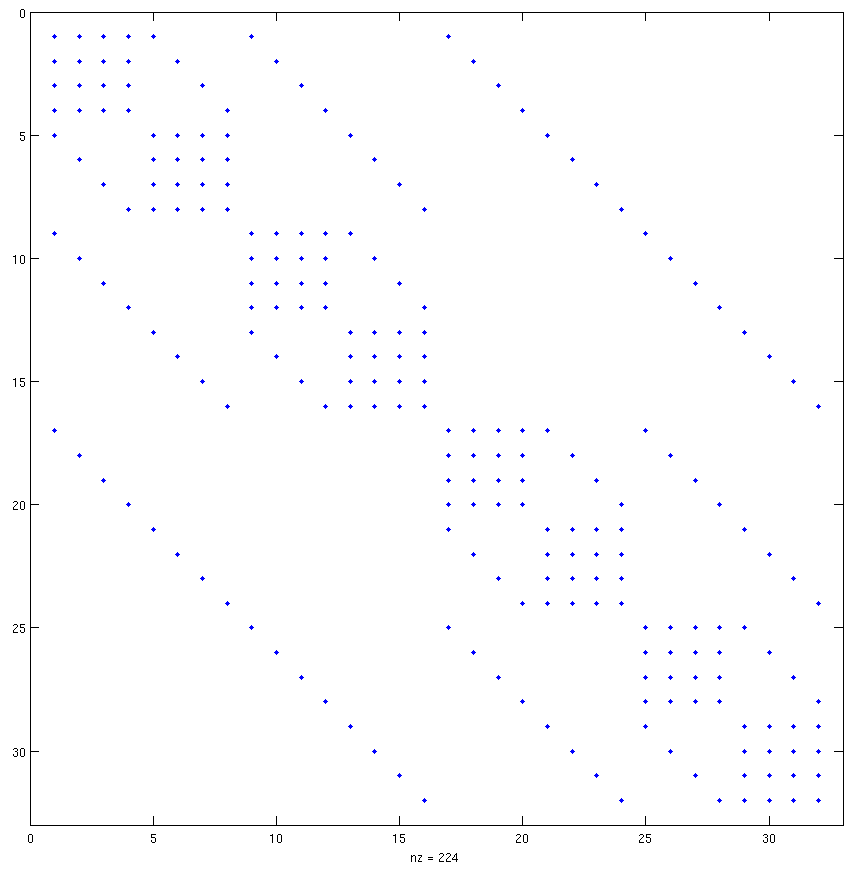
\includegraphics[width=3.25in]{chapters/spn_equations/group1.png}
  \end{center}
  \caption{\textbf{Sparsity pattern for 1-group $SP_7$
      discretization.} \textit{A $2\times 2 \times 2$ element mesh was
      used to show detail of the blocks formed by the discretization.}}
  \label{fig:group1}
\end{figure}
\begin{figure}[t!]
  \begin{center}
    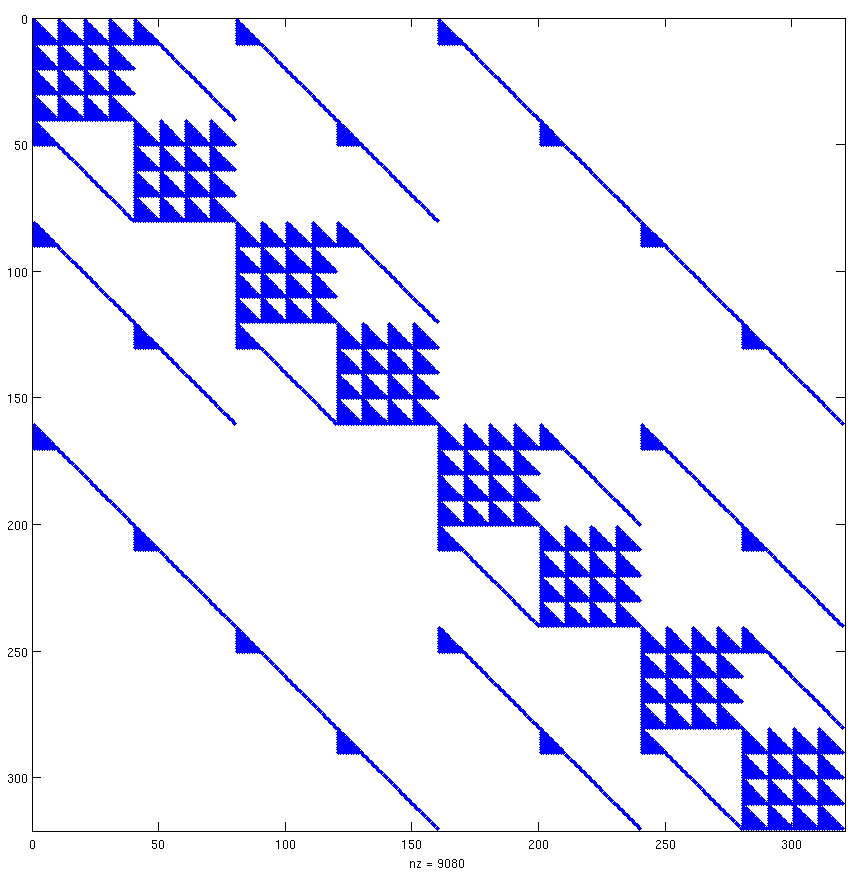
\includegraphics[width=3.25in]{chapters/spn_equations/group10ds.png}
  \end{center}
  \caption{\textbf{Sparsity pattern for 10-group $SP_7$ discretization
      with downscatter only.} \textit{A $2\times 2 \times 2$ element
      mesh was used to show detail of the blocks formed by the
      discretization.}}
  \label{fig:group10ds}
\end{figure}
\begin{figure}[t!]
  \begin{center}
    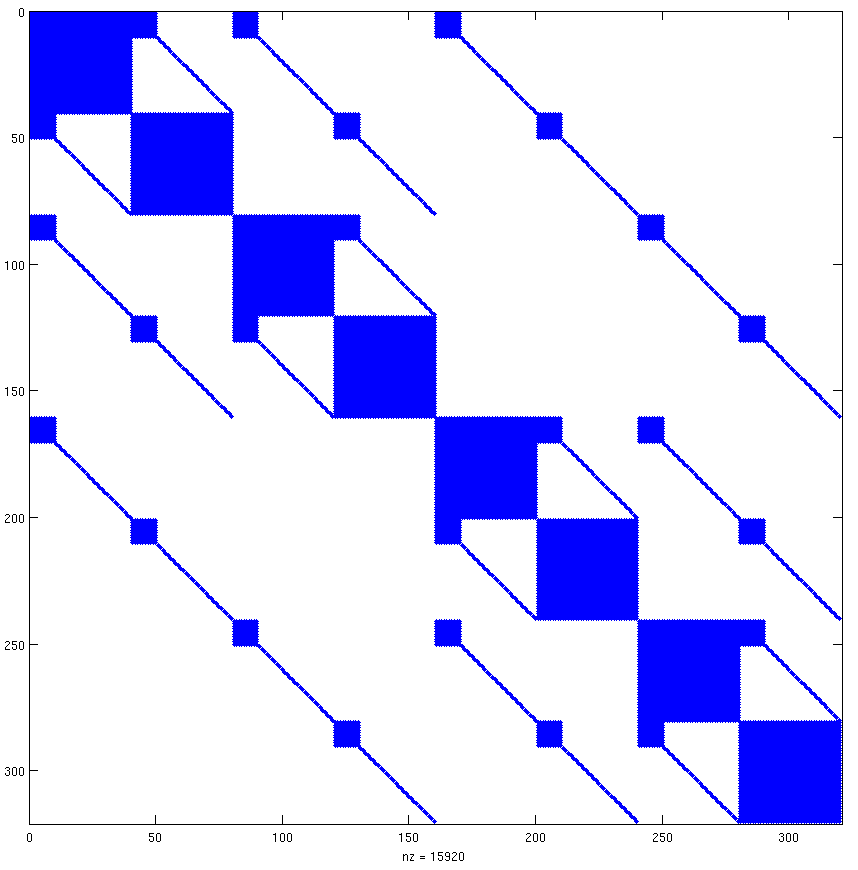
\includegraphics[width=3.25in]{chapters/spn_equations/group10us.png}
  \end{center}
  \caption{\textbf{Sparsity pattern for 10-group $SP_7$ discretization
      with downscatter and upscatter.} \textit{A $2\times 2 \times 2$ element
      mesh was used to show detail of the blocks formed by the
      discretization.}}
  \label{fig:group10us}
\end{figure}
We note a few key features of the sparsity plots. The first is that
for multigroup problems without full upscatter and downscatter
(i.e. Figure~\ref{fig:group10ds}), the resulting matrix is asymmetric
and therefore a linear solver that can handle asymmetric linear
systems is required. Nearly all problems of interest will not have
full upscattering or downscattering. Second we note the largely
diagonal character of these systems, although the blocks from
Eq~(\ref{eq:A_block_matrix}) are readily apparent. 

Based on this both block and diagonally dominant structure for
matrices formed by the general multigroup $SP_N$ equations, we choose
\textit{block Jacobi} preconditioning as a left preconditioner for the
system. Block Jacobi preconditioning extracts the diagonal elements of
the matrix as the preconditioner where now the elements extracted are
the blocks on the diagonal as shown on the left side of
Figure~\ref{fig:block_jacobi_ex}. Shown on the right side of
Figure~\ref{fig:block_jacobi_ex}, inversion of the preconditioner is
trivial with each diagonal block inverted separately. For the $SP_N$
equations, Eq~(\ref{eq:A_block_matrix}) gives a block size of
$N_g\times(N+1)/2$.
\begin{figure}[t!]
  \begin{center}
    \scalebox{1.5}{
    \input{chapters/spn_equations/block_jacobi.pdftex_t} }
  \end{center}
  \caption{\textbf{Block Jacobi preconditioning strategy used for the
      $SP_N$ equations.} \textit{Left: The preconditioner is formed by
      the diagonal blocks of the matrix. Right: Inversion of the
      preconditioner is trivial and decoupled by block.}}
  \label{fig:block_jacobi_ex}
\end{figure}

For high performance implementations this has several attractive
properties. First, the blocks in the matrix come from the energy/angle
discretization of the transport equation as given by
Eq~(\ref{eq:A_block_matrix}). Each block on the diagonal is bound to a
mesh element in the system (note there are 8 blocks on the diagonal in
each of the sparsity patterns with a mesh of $2 \times 2 \times 2$)
and therefore we expect the matrix elements forming the block to be
entirely local in domain decomposed calculations. Second, these blocks
are typically dense and nearly lower triangular for many transport
problems meaning that established dense matrix methods can be used for
fast inversion.

Spectral radius computations for the block Jacobi preconditioned
iteration matrix were performed with Table~\ref{tab:group1bj} giving
the results for the 1-group case, Table~\ref{tab:group10dsbj} for the
10-group case with full downscatter only and
Table~\ref{tab:group10usbj} for the 10-group case with full
downscatter and full upscatter. A block size of $N_g\times(N+1)/2$ was
used for the preconditioner in all cases.
\begin{table}[h!]
  \begin{center}
    \begin{tabular}{cccccc}\hline\hline
      \multicolumn{1}{c}{}& 
      \multicolumn{1}{c}{}& 
      \multicolumn{1}{c}{}& 
      \multicolumn{1}{c}{$SP_N$ Order}& 
      \multicolumn{1}{c}{}& 
      \multicolumn{1}{c}{} \\
       &   & \textbf{1} & \textbf{3} & \textbf{5} & \textbf{7}  \\
       & \textbf{0} & 0.0635 & 0.1269 & 0.1444 & 0.1513 \\
       & \textbf{1} & 0.0666 & 0.1315 & 0.1474 & 0.1534 \\
      $P_N$ Order & \textbf{3} & 0.0666 & 0.1365 & 0.154 & 0.1592 \\
       & \textbf{5} & 0.0666 & 0.1365 & 0.1562 & 0.163 \\
       & \textbf{7} & 0.0666 & 0.1365 & 0.1562 & 0.164 \\
      %%
      \hline\hline
    \end{tabular}
  \end{center}
  \caption{\textbf{Spectral radius results for the block Jacobi
      preconditioned iteration matrix with 1 energy group.}}
  \label{tab:group1bj}
\end{table}
\begin{table}[h!]
  \begin{center}
    \begin{tabular}{cccccc}\hline\hline
      \multicolumn{1}{c}{}& 
      \multicolumn{1}{c}{}& 
      \multicolumn{1}{c}{}& 
      \multicolumn{1}{c}{$SP_N$ Order}& 
      \multicolumn{1}{c}{}& 
      \multicolumn{1}{c}{} \\
       &   & \textbf{1} & \textbf{3} & \textbf{5} & \textbf{7}  \\
       & \textbf{0} & 0.0647 & 0.1275 & 0.1449 & 0.1514 \\
       & \textbf{1} & 0.0686 & 0.1338 & 0.1484 & 0.1547 \\
      $P_N$ Order & \textbf{3} & 0.0687 & 0.1399 & 0.1582 & 0.1625 \\
       & \textbf{5} & 0.0692 & 0.1399 & 0.1582 & 0.1657 \\
       & \textbf{7} & 0.0678 & 0.1393 & 0.1624 & 0.166 \\
      %%
      \hline\hline
    \end{tabular}
  \end{center}
  \caption{\textbf{Spectral radius results for the block Jacobi
      preconditioned iteration matrix with 10 energy groups and full
      downscatter.}}
  \label{tab:group10dsbj}
\end{table}
\begin{table}[h!]
  \begin{center}
    \begin{tabular}{cccccc}\hline\hline
      \multicolumn{1}{c}{}& 
      \multicolumn{1}{c}{}& 
      \multicolumn{1}{c}{}& 
      \multicolumn{1}{c}{$SP_N$ Order}& 
      \multicolumn{1}{c}{}& 
      \multicolumn{1}{c}{} \\
       &   & \textbf{1} & \textbf{3} & \textbf{5} & \textbf{7}  \\
       & \textbf{0} & 0.1887 & 0.2267 & 0.2285 & 0.2286 \\
       & \textbf{1} & 0.4535 & 0.5044 & 0.5045 & 0.5045 \\
      $P_N$ Order & \textbf{3} & 0.4535 & 0.6453 & 0.6506 & 0.6506 \\
       & \textbf{5} & 0.4535 & 0.6453 & 0.6802 & 0.6818 \\
       & \textbf{7} & 0.4535 & 0.6453 & 0.6802 & 0.6927 \\
      %%
      \hline\hline
    \end{tabular}
  \end{center}
  \caption{\textbf{Spectral radius results for the block Jacobi
      preconditioned iteration matrix with 10 energy groups, full
      downscatter and full upscatter.}}
  \label{tab:group10usbj}
\end{table}

From the tabulated block Jacobi data it is clear that this is a viable
preconditioning choice for all $SP_N$ problems in terms of Monte Carlo
solution methods. All cases were observed to have a spectral radius
below unity. Based on these results, the block Jacobi method should be
the applicable to more complicated problems representative of physical
nuclear systems.

%%---------------------------------------------------------------------------%%
\section{Fuel Assembly Criticality Calculations}
\label{sec:fuel_assembly_calcs}
Fuel assembly calculations are a critical piece of nuclear engineering
infrastructure for reactor core analysis and design. At this level,
individual fuel pins may be resolved at fine resolution in a variety
of configurations. As a sophisticated problem of interest to push the
limits of MCSA, a hot zero-power $17 \times 17$ pin assembly will be
used with varying energy group structure and $SP_N$ discretization in
a criticality calculation. A cross section along the vertical axis
showing homogenized fuel pin, control rod, and moderator materials and
the associated grid is given by Figure~\ref{fig:problem3_radial_mat}
while a cross section of the materials configuration along the
horizontal axis is given by Figure~\ref{fig:problem3_axial_mat}. A
detailed view of the assembly bottom is given in
Figure~\ref{fig:problem3_end}. On the top and bottom of the assembly,
vacuum conditions are used as well as on the top and right boundaries
in Figure~\ref{fig:problem3_radial_mat}. Reflecting conditions are
used on the left and bottom boundaries of
Figure~\ref{fig:problem3_radial_mat}, effectively giving a
representation of one quarter of the assembly. For the spatial
discretization, each fuel pin (gray regions in
Figure~\ref{fig:problem3_radial_mat}) is resolved by a $2 \times 2$
mesh with materials and cross sections homogenized over this region.
\begin{figure}[t!]
  \begin{center}
    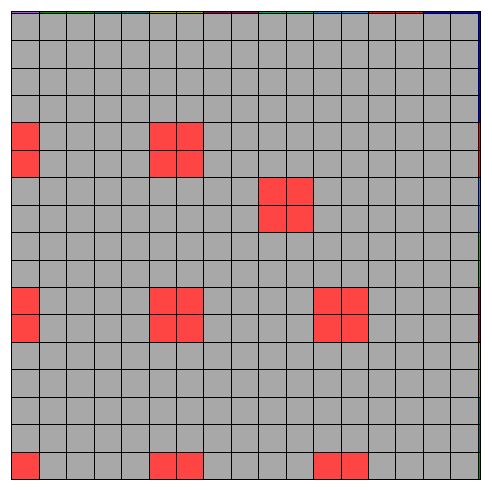
\includegraphics[width=4in]{chapters/spn_equations/problem3_radial_mat.png}
  \end{center}
  \caption{\textbf{Fuel assembly mesh and geometry cross section.}
    \textit{Reflecting boundaries are used on the left and lower
      boundaries to create a complete $17 \times 17$ assembly
      geometry. Gray regions are homogenized fuel and red regions are
      homogenized control rods. The control rods were removed for
      these problems. Each fuel pin is resolved by a $2 \times 2$
      mesh.}}
  \label{fig:problem3_radial_mat}
\end{figure}
\begin{figure}[t!]
  \begin{center}
    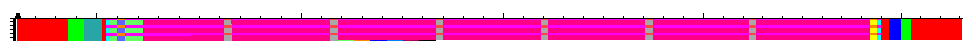
\includegraphics[width=6.0in]{chapters/spn_equations/problem3_axial_mat.png}
  \end{center}
  \caption{\textbf{Fuel assembly geometry cross section.} \textit{The
      geometry is subdivided along the axial direction into 50 zones
      spaced to capture material boundaries. Important details include
      spacer grids along the length of the fuel pins and reactor core
      structures on the top and bottom of the assembly. Lighter purple
      material in the center of the assembly is moderator and darker
      purple/red material is fuel.}}
  \label{fig:problem3_axial_mat}
\end{figure}
\begin{figure}[t!]
  \begin{center}
    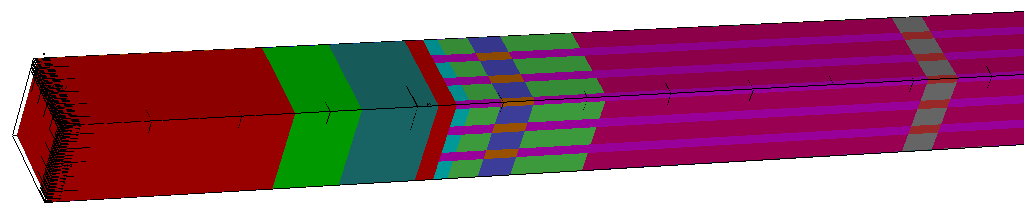
\includegraphics[width=6.0in]{chapters/spn_equations/problem3_end.png}
  \end{center}
  \caption{\textbf{Fuel assembly geometry end detail.}
    \textit{Reactor core structure including spacer grids and plenum
      has been included. Lighter purple material on the right of the
      figure is moderator and darker purple/red material is fuel.}}
  \label{fig:problem3_end}
\end{figure}

Significant geometric details are contained in the model including
spacer grids, fuel pins with homogenized cladding and gas gap, core
plenum, and moderator with boron. Group cross sections and other
discrete nuclear data are generated as needed by a cross-section
processing module dependent on the meshing parameters used to
discretize the geometry and single-dimension pin-cell calculations for
initial flux spectrum generation. Table~\ref{tab:problem3_parameters}
gives the primary design parameters for the fuel assembly
calculations.
\begin{table}[h!]
  \begin{center}
    \begin{tabular}{ll}\hline\hline
      \multicolumn{1}{l}{\textbf{Parameter}} & 
      \multicolumn{1}{l}{\textbf{Value}} \\
      Power Level & 0 MW \\
      Inlet Temperature & 326.85C \\
      Fuel Temperature & 600C \\
      Boron Concentration & 1300 ppm \\
      Moderator Density & 0.743 g/cc \\
      Helium Density & \sn{1.79}{-4} g/cc \\
      Zirconium Density & 6.56 g/cc \\
      Stainless Steel Density & 8.0 g/cc \\
      Inconel Density & 8.19 g/cc \\
      UO2 Density & 10.257 g/cc \\
      Fuel Pin Radius (w/o clad) & 0.4096 cm \\
      %%
      \hline\hline
    \end{tabular}
  \end{center}
  \caption{\textbf{Design parameters for the $17 \times 17$ pin fuel
      assembly criticality calculation.}}
  \label{tab:problem3_parameters}
\end{table}

To generate the multiplication factor and steady-state flux
distribution for this problem, at every eigenvalue iteration MCSA is
used to solve the resulting $SP_N$ problem using the provided fission
source. Algorithm~\ref{alg:power_iteration} presents the use of MCSA
within a power iteration strategy to find the multiplication factor.
\begin{algorithm}[h!]
  \caption{Power Iteration MCSA Scheme}
  \label{alg:power_iteration}
  \begin{algorithmic}
    \State $k_0 =$ initial guess
    \State $\mathbf{\Phi}_0 =$ initial guess
    \State $n = 0$
    \While{$|\frac{k^n - k^{n-1}}{k^n}| < \epsilon$}
    \Comment{Iterate until convergence of the eigenvalue}
    \State $\mathbf{M} \mathbf{\Phi}^{n+1} = \frac{1}{k^n} \mathbf{F} \mathbf{\Phi}^n$
    \Comment{Solve for the new flux state with MCSA}
    \State $k^{n+1} = k^n \frac{\int \mathbf{F} \mathbf{\Phi}^{n+1} d\mathbf{r}}{\int
      \mathbf{F} \mathbf{\Phi}^n d\mathbf{r}}$
    \Comment{Update the multiplication factor}
    \State $n = n+1$
    \EndWhile
  \end{algorithmic}
\end{algorithm}
Here, $\mathbf{M}$ is the transport operator generated on the
left-hand side of the $SP_N$ discretization, $\mathbf{F}$ is the
fission matrix, and $\mathbf{\Phi}$ the multigroup neutron flux. This
problem is significantly more complicated than the simple test problem
used for the previous spectral analysis. Fission has been introduced
into the set of equations and the addition of moderator into the
system will increase the amount of scattering, creating a
significantly more difficult problem manifesting itself in an
iteration matrix with a larger spectral radius. When using MCSA, the
linear operator applied to $\mathbf{\Phi}^{n+1}$ at each eigenvalue
iteration will dictate convergence and remain unchanged throughout the
eigenvalue computation while the addition of fission to the system
will only modify the source of neutrons and the multiplication factor
at every eigenvalue iteration while not affecting Monte Carlo
transport.
 
\subsection{Preliminary Jacobi Preconditioned Calculations}
\label{subsec:jacobi_prec_assembly_calc}
We first use block Jacobi preconditioning to solve the $17 \times 17$
fuel assembly problem. A single energy group problem was first
computed with $SP_1$ discretization, effectively giving the one-speed
neutron diffusion system for the fuel assembly resulting in 20,088
degrees of freedom in the
problem. Figure~\ref{fig:block_jacobi_res_mcsa} gives the residual
infinity norm as a function of iteration for the MCSA linear solve in
the first eigenvalue iteration using 25,000 stochastic histories at
every iteration for the adjoint Neumann-Ulam solve.
\begin{figure}[t!]
  \begin{center}
    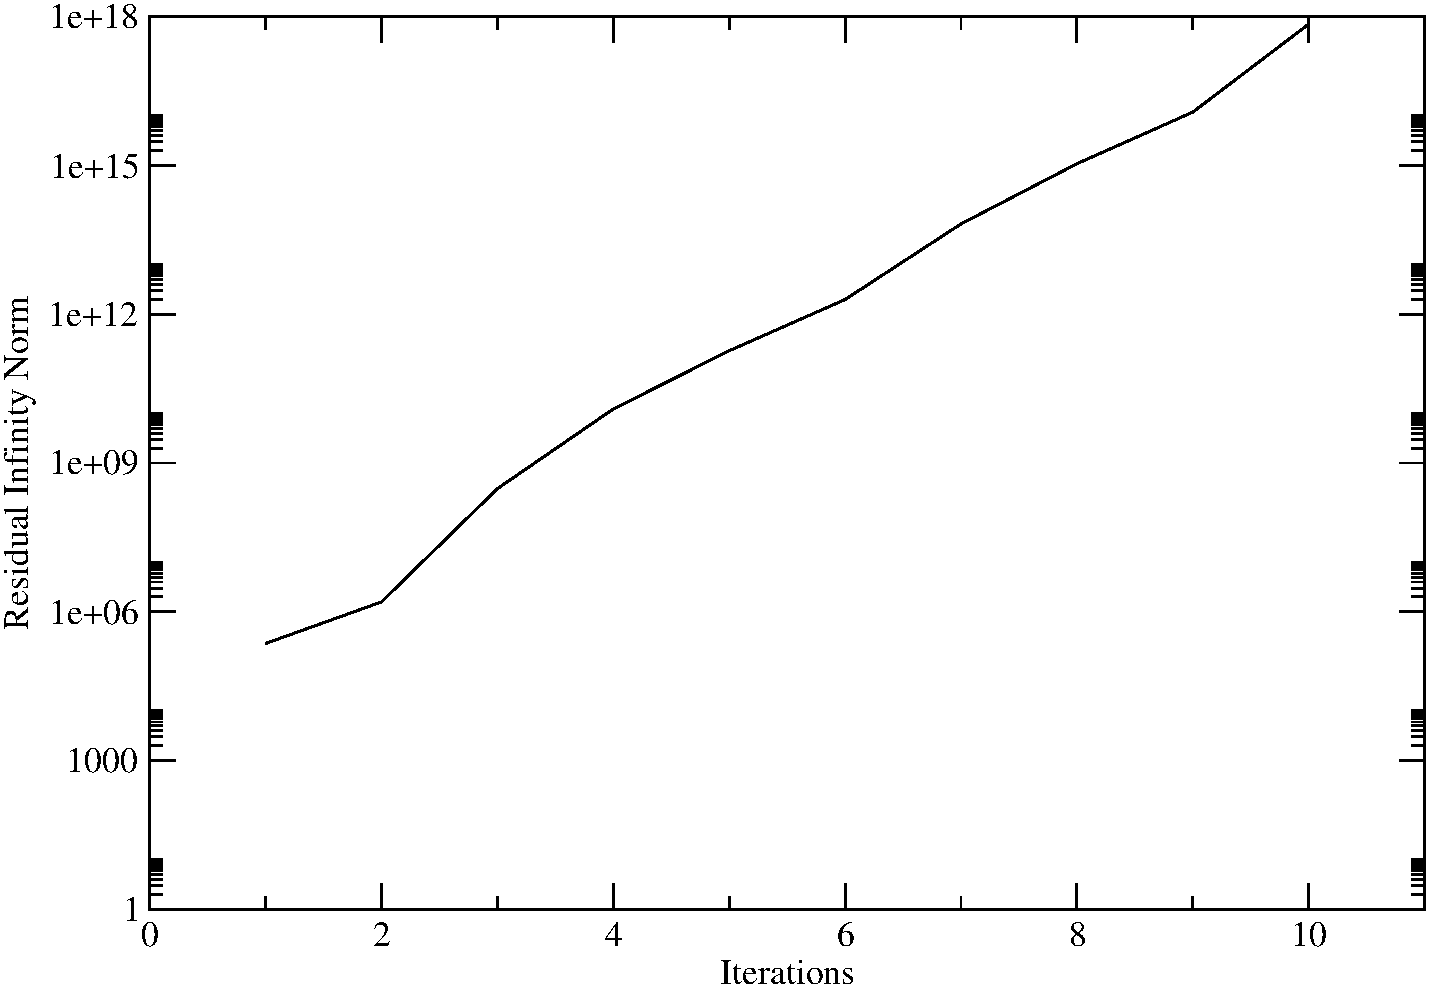
\includegraphics[width=5in]{chapters/spn_equations/block_jacobi_res.pdf}
  \end{center}
  \caption{\textbf{Residual infinity norm vs. iteration for the block
      Jacobi preconditioned MCSA solve during the first eigenvalue
      iteration of the 1-group $17 \times 17$ fuel assembly problem.}
    \textit{Convergence was not achieved with the block Jacobi
      preconditioned method.}}
  \label{fig:block_jacobi_res_mcsa}
\end{figure}
Convergence was not achieved as noted by the rapid rise in the
residual over a few iterations. Based on the spectral radius
computations performed, these results are not in line with
expectations for this problem. Additional computations performed with
\sn{1}{6} histories per iteration exhibited the same divergent
behavior at a significant computational cost and compute time. Even if
the problem may be ill-conditioned, we do expect convergence of MCSA
given that the spectral radius requirement was met. To investigate
further, a block Jacobi preconditioned Richardson iteration was used
to solve the same
problem. Figure~\ref{fig:block_jacobi_res_richardson} gives the
residual infinity norm as a function of iteration for the Richardson
linear solve in the first eigenvalue iteration.
\begin{figure}[t!]
  \begin{center}
    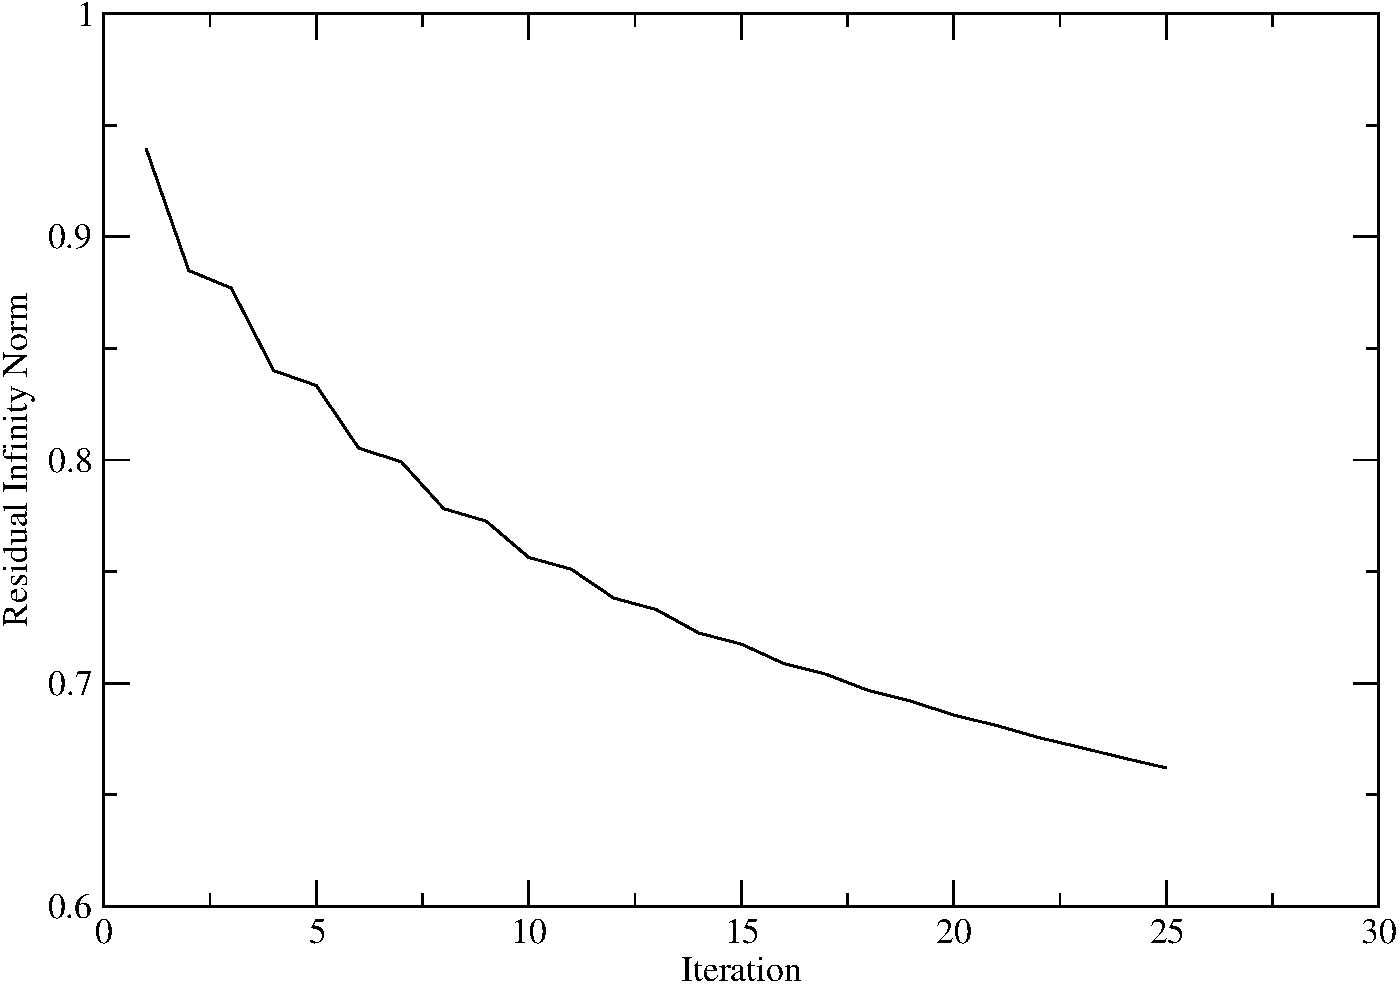
\includegraphics[width=5in]{chapters/spn_equations/block_jacobi_rich_res.pdf}
  \end{center}
  \caption{\textbf{Residual infinity norm vs. iteration for the block
      Jacobi preconditioned Richardson solve during the first
      eigenvalue iteration of the 1-group $17 \times 17$ fuel assembly
      problem.} \textit{A spectral radius near 1 was observed for the
      iteration matrix.}}
  \label{fig:block_jacobi_res_richardson}
\end{figure}
Poor convergence is observed for the Richardson iteration, however,
convergence is achieved meaning that the preliminary eigenvalue
criteria needed to satisfy MCSA convergence has also been met. The
number of iterations required for the Richardson iteration to converge
will give an approximation for the spectral radius via
Eq~(\ref{eq:linear_k_iter_norm3}). With 7291 iterations required to
converge to a tolerance of $\sn{1}{-6}$, $\rho(\mathbf{H}) \approx
0.998$, nearing the limits of MCSA applicability and well beyond the
spectral radii generated in the initial spectral analysis.

Based on these results, it then appears that even if the simple
criteria of a spectral radius of less than one is met and the
Richardson iteration will converge with the same preconditioning, MCSA
still may not converge. We then expect the issue to reside with the
Neumann-Ulam solve providing the correction as the Richardson
iteration is known to provide the correct result. Furthermore, the
fact that the spectral radius is less than one means that the
stochastic histories in the block Jacobi preconditioned Neumann-Ulam
method are eventually being terminated by the weight cutoff as no
artificial absorption was used for these preliminary
calculations. Based on this, the correction being generated by the
Neumann-Ulam solve is the component of MCSA causing a divergent
solution.

\subsection{MCSA Breakdown}
\label{subsec:mcsa_break_down}
For the fuel assembly problem, the initial block Jacobi preconditioned
calculations used a one-speed $SP_1$ discretization, effectively
giving a diffusion system. To study the breakdown of MCSA at iteration
matrix spectral radii near one, we will use the simpler homogeneous
2-dimensional one-speed neutron diffusion system presented in
Appendix~\ref{chap:diffusion_problem} to isolate this behavior. In
this system, we can vary the cross sections while maintaining a fixed
grid in order to achieve varying spectral radii. For these studies, we
neglect fission as MCSA behavior is dictated by the transport operator
$\mathbf{M}$ in an eigenvalue scheme with the fission matrix used to
generate a fixed source.

For each solver and estimator combination, the spectral radius of the
iteration matrix generated by the diffusion problem was varied by
changing the absorption cross section from 0.25 to 100 while fixing
the grid size at $100 \times 100$ with $h = 0.1$ and a fixed
scattering cross section of unity. For each parameter variation, a
minimum of one stochastic history per degree of freedom (DOF) in the
problem was used to compute the Monte Carlo correction. If the solver
could not converge in less than 100 iterations, the number of
histories was increased by increments of 5,000 until convergence was
achieved in less than 100 iterations. The number of iterations
required to converge MCSA and the time to converge was recorded as a
means to capture the breakdown.

Figure~\ref{fig:breakdown_iterations} gives the number of iterations
required to converge for the chosen number of histories per iteration
given by Figure~\ref{fig:breakdown_histories} using the adjoint solver
with the collision and expected value estimators and the forward
solver with the collision estimator. For spectral radii less than
0.97, all MCSA problems converged with 1 history per DOF (10,000 for
this problem) with the number of iterations required to converge
increasing as a function of spectral radius. Near a spectral radius of
0.97, the number of histories required to converge MCSA in less than
100 iterations takes a dramatic rise that exhibits neither exponential
nor power law behavior. As the spectral radius approaches 1, the
number of histories required becomes significant and effectively
impractical to compute. Even with this simple diffusion problem, the
behavior is consistent with that observed for the fuel assembly
problem with $SP_1$ discretization. In that case, we estimated a
spectral radius of $\approx 0.998$, larger than any of the spectral
radii that could be computed within even 90 minutes of compute time
for this simple two dimensional problem. For that problem, even
1,000,000 histories ($\approx 50$ per DOF) was not enough to provide
convergence. Even if single solve times of an hour can be tolerated,
dozens of solves are typically required to compute the multiplication
factor and flux spectrum within the $SP_N$ eigenvalue scheme for more
difficult problems like the fuel assembly, making the method unusable.
\begin{figure}[t!]
  \begin{center}
    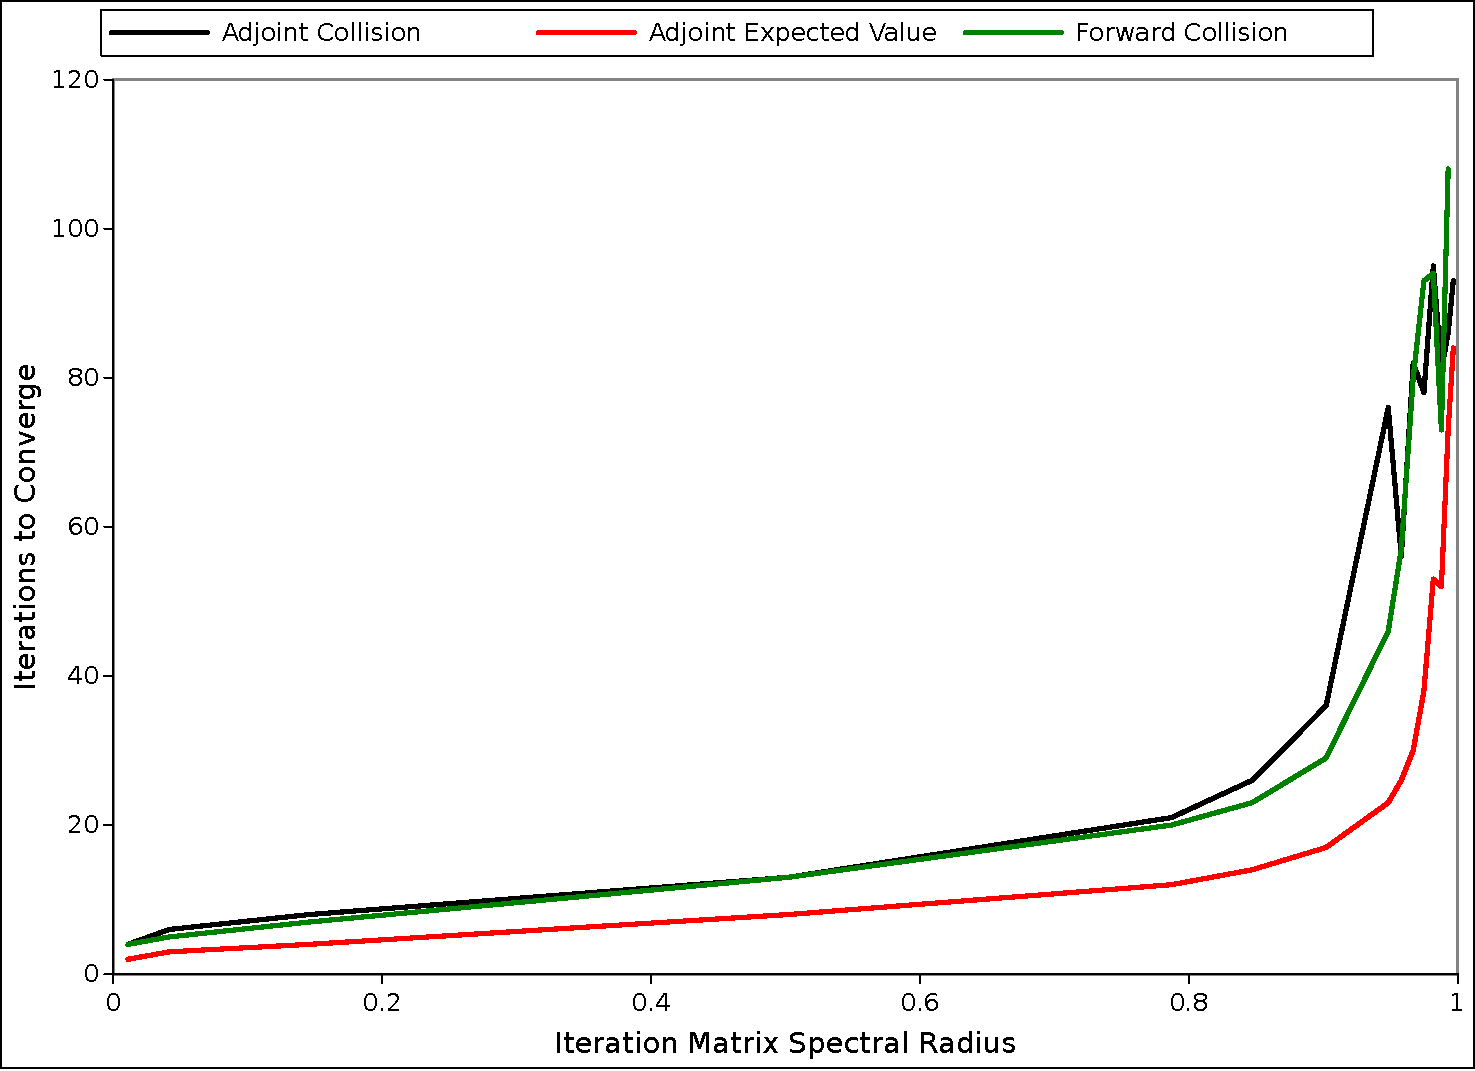
\includegraphics[width=4.25in]{chapters/spn_equations/breakdown_iterations.pdf}
  \end{center}
  \caption{\textbf{Iterations required to converge as a function of
      spectral radius for the neutron diffusion problem.} \textit{The
      number of histories was increased to achieve convergence in less
      than 100 iterations. At least 10,000 histories were used for
      each calculation.}}
  \label{fig:breakdown_iterations}
\end{figure}
\begin{figure}[t!]
  \begin{center}
    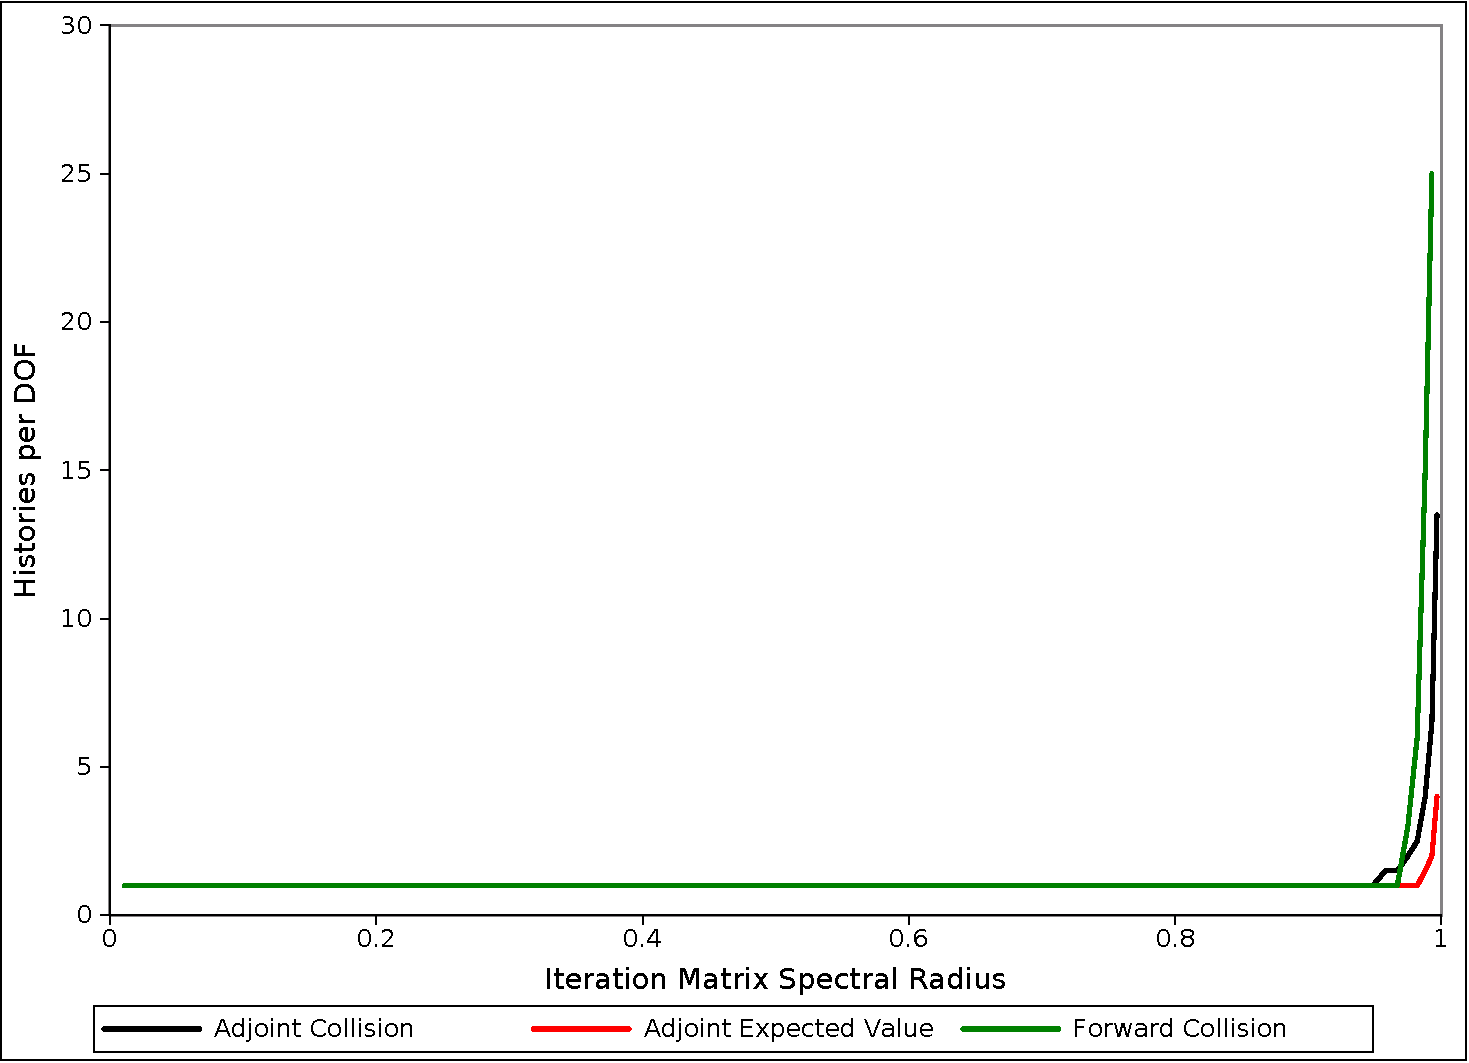
\includegraphics[width=4.25in]{chapters/spn_equations/breakdown_histories.pdf}
  \end{center}
  \caption{\textbf{Histories per DOF required to converge as a
      function of spectral radius for the neutron diffusion problem.}
    \textit{The number of histories was increased to achieve
      convergence in less than 100 iterations. At least 10,000
      histories were used for each calculation with 10,000 DOFs in the
      problem.}}
  \label{fig:breakdown_histories}
\end{figure}

In addition to the significantly larger number of histories required
to achieve convergence for ill-conditioned problems another penalty is
paid due to histories that take longer to
compute. Figure~\ref{fig:breakdown_time} gives the CPU time in seconds
required to compute a single random walk averaged over the entire set
of histories run in the calculation over all iterations. As the
spectral radius increases (correlating to a higher ratio of scattering
in the system) the random walk lengths increase, using more CPU time
to finish the computation. Compared to spectral radii of 0.5, larger
spectral radii over 0.97 have histories that require two orders of
magnitude more computation time. This significant increase in
computation time per history coupled with the significant increase in
the number of histories required to converge is evidence that for
problems with spectral radii above $\approx 0.97$, using MCSA to solve
any problems of interest is entirely ineffective and not practical. At
iteration matrix spectral radii this large, using significant numbers
of stochastic histories in the Monte Carlo solve are not enough to
reduce the stochastic uncertainty in the correction, causing the MCSA
sequence to diverge instead of accelerating convergence. We therefore
require a more expansive set of preconditioning techniques to move the
eigenvalue spectrum of the $SP_N$ problem into a regime in which MCSA
is more applicable and in which performance is improved.
\begin{figure}[t!]
  \begin{center}
    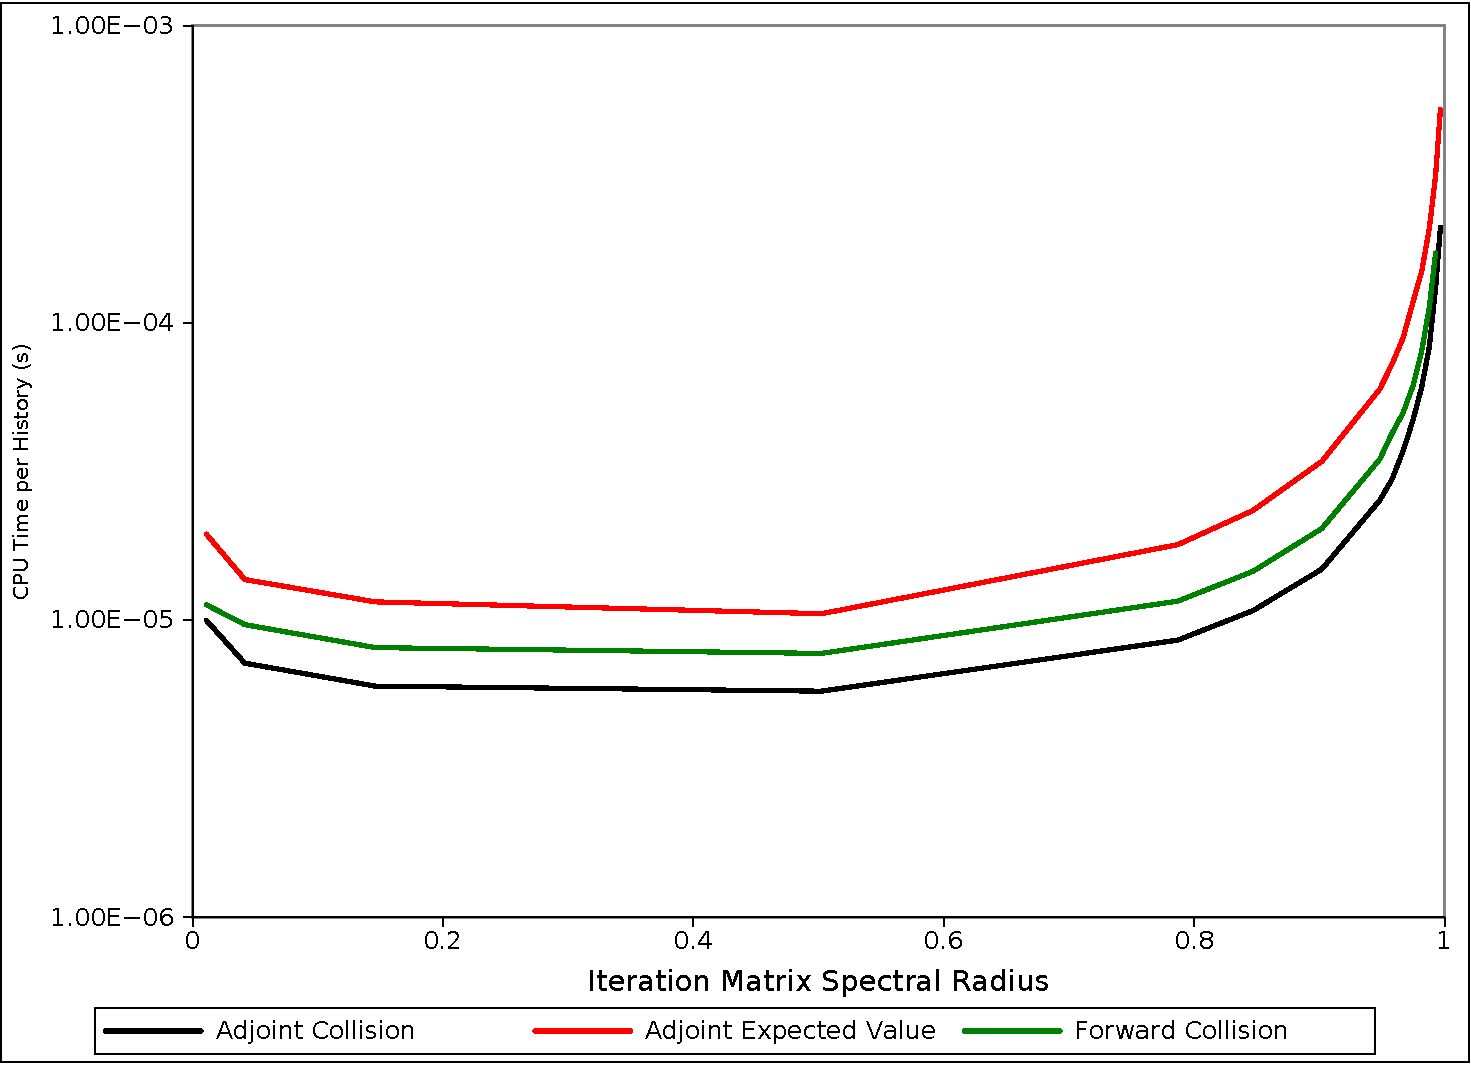
\includegraphics[width=4.25in]{chapters/spn_equations/breakdown_time.pdf}
  \end{center}
  \caption{\textbf{CPU time per history as a function of spectral
      radius for the neutron diffusion problem.} \textit{As the
      spectral radius grows, so do the length of the random
      walks. Longer random walks require more CPU time to compute.}}
  \label{fig:breakdown_time}
\end{figure}

\clearpage

%%---------------------------------------------------------------------------%%
\section{Advanced Preconditioning Strategies}
\label{subsec:spn_advanced_preconditioning}
For the fuel assembly criticality problem presented in the previous
section, the spectral radius was near one using Jacobi preconditioning
and in a regime in which MCSA breakdown is observed. In this regime
the number of stochastic histories required to converge MCSA increases
rapidly and the resulting poor performance is compounded by those
histories being increasingly expensive to compute. To overcome this
difficulty, advanced preconditioning strategies for the $SP_N$ problem
are required beyond simple Jacobi methods that can reduce the spectral
radius into a region of better MCSA performance. Two modern algebraic
preconditioning strategies, ILUT and SPAINV, will be presented here
and used within the explicit preconditioning framework given by
Eq~(\ref{eq:left_right_mcsa}). Data
showing their effects on MCSA solutions of the fuel assembly
criticality problem will be presented.

\subsection{ILUT Preconditioning}
\label{subsec:spn_ilut_preconditioning}
ILUT preconditioning is chosen due to its applicability to problems
that have a dominating elliptic compoenent such as the fuel assembly
problem and because it is easily formulated algebraicly. Incomplete
lower-upper (ILU) factorizations of the linear operator can be used a
simple mechanism to form an approximate inverse of a
preconditioner. To build the factorization, the sparse upper and lower
triangular factors, $\mathbf{L}$ and $\mathbf{U}$, are computed such
that the residual matrix formed by the factorization
\cite{saad_iterative_2003}:
\begin{equation}
  \mathbf{R} = \mathbf{L} \mathbf{U} - \mathbf{A} \:,
  \label{eq:ilu_residual_matrix}
\end{equation}
has a specified sparsity pattern and element magnitude. When a
magnitude threshold is used, elements generated in the factors below
that magnitude are dropped, resulting in ILU threshold (ILUT)
preconditioning. The sparsity pattern in this case is determined from
the input matrix to be preconditioned and the number of elements
maintained in the factor is specified by a fill level parameter. A
fill level of 1 will generate the same number of elements as the
sparsity pattern of the input matrix while a fill level of 2 will
contain twice as many elements in the factorization, resulting in a
better representation of the true LU factorization. The inverse of the
lower and upper triangular factors may then be easily inverted by
means of simple elimination to produce the preconditioner. For MCSA,
$\mathbf{L}^{-1}$ will be used on the left and $\mathbf{U}^{-1}$ on
the right to precondition the system.

For modern subspace methods, only the action to the preconditioner on
a vector is required for efficient implementations and therefore a
triangular solve can be used for this purpose. For the explicit
preconditioning scheme presented in Eq~(\ref{eq:left_right_mcsa}), the
fully inverted operator must be generated in order to build the set of
probabilities and weights required for Monte Carlo
sampling. Therefore, for a linear system of size $N$, $N$ triangular
solves will be required in order to extract the inverse matrices from
production ILU implementations. In addition, parallel implementations
typically generate lower and upper factors that are only triangular
locally, providing an easily parallelizable mechanism to generate the
action of the preconditioner inverse. A consequence of this choice for
parallel scalability is a degradation of the preconditioning quality
as the size of the parallel system is increased. For serial
computations, the triangular factorization is potentially exact
depending on the parameters chosen while at thousands of parallel
tasks, the global triangular factors differ significantly from the true
factorization. As a result, more iterations are required at higher
levels of parallelism to converge the system and will ultimately
degrade overall scalability of the system with respect to total wall
time to converge.

MCSA preconditioned with ILUT was used to solve the fuel assembly
problem presented in the previous section for a 1-group $SP_1$
discretization. Unlike the Jacobi preconditioned strategy, convergence
was achieved with ILUT preconditioning. To study convergence
sensitivity to ILUT parameters, the fill level and drop tolerance were
parametrically varied with the number of iterations to converge an
eigenvalue iteration for the fuel assembly problem recorded along with
the maximum number of non-zero entries observed in all matrix rows for
the left/right preconditioned composite linear operator. To provide
some sparsity to the factorization, the ILUT drop tolerance was used
to drop elements in the extracted inverse triangular factors. For each
calculation, the number of iterations required to converge reported
was for a single eigenvalue iteration with \sn{3}{4} histories at each
MCSA iteration to compute the Monte Carlo correction using the adjoint
collision estimator. All ILUT calculations reported here were
performed on a single CPU and therefore this data does not take into
account the aforementioned effects of parallel decomposition on the
quality of the ILUT preconditioning.

Figure~\ref{fig:ilut_iterations} gives the number of iterations to
converge the fixed source problem to a tolerance of \sn{1}{8}. As
expected, the higher the fill level chosen for the ILUT factorization,
the fewer iterations are required to converge the problem (only 9 MCSA
iterations were required to converge the problem for the fill level of
3 and drop tolerance of \sn{1}{-5} case). For higher levels of fill,
the iterations needed to converge were not as sensitive, signaling
that a larger drop tolerance can perhaps be used without a significant
degradation in iterative performance. At smaller fill levels, the
sensitivity to the ILUT drop tolerance is more significant. For all
fill levels used, convergence was not achieved for the fuel assembly
problem with a drop tolerance larger than \sn{1}{-3}.
\begin{figure}[t!]
  \begin{center}
    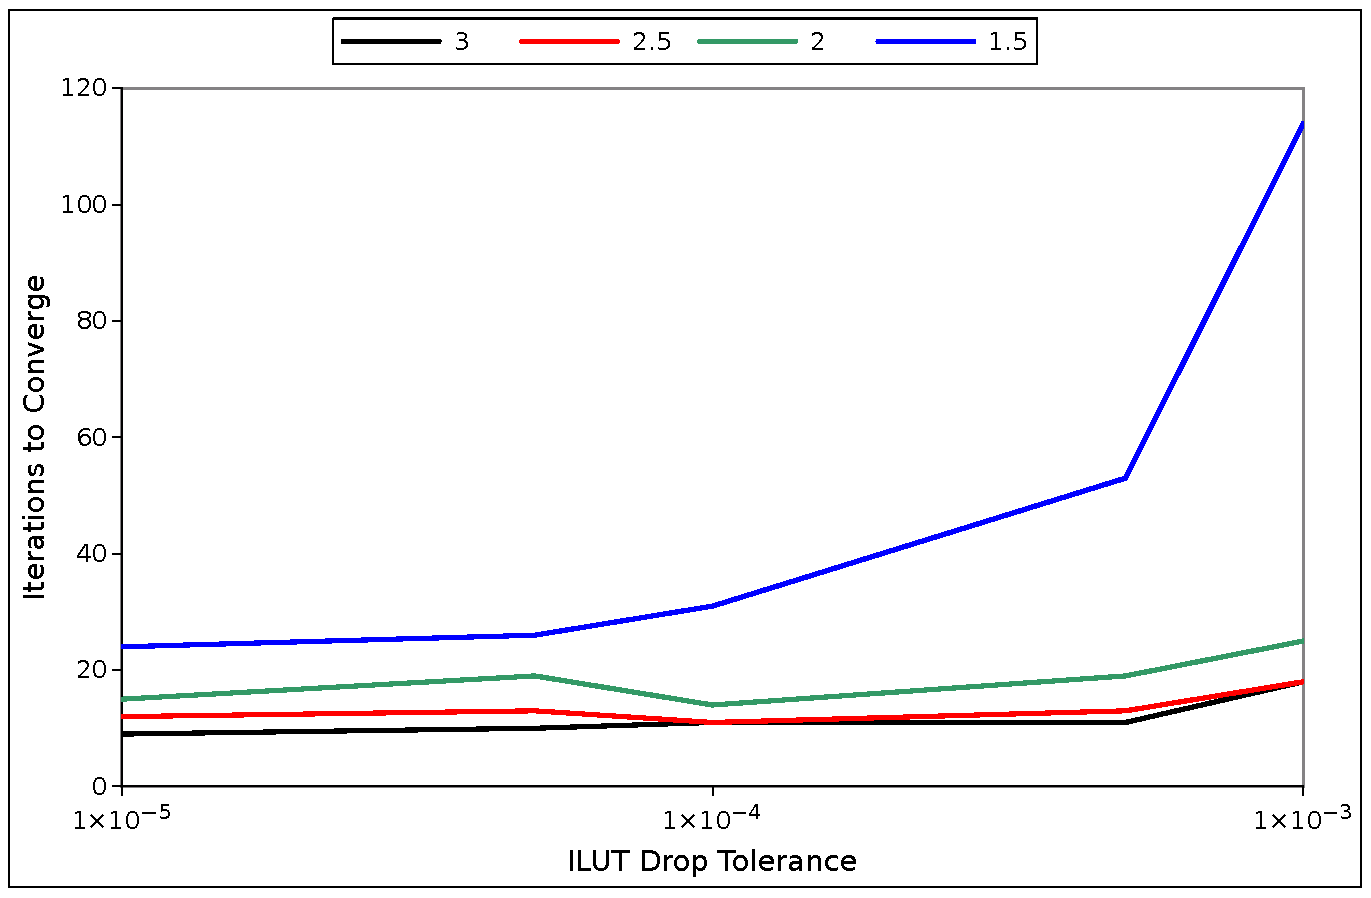
\includegraphics[width=4.25in]{chapters/spn_equations/ilut_iterations.pdf}
  \end{center}
  \caption{\textbf{Number of MCSA iterations required to converge an
      eigenvalue iteration for the fuel assembly problem with ILUT
      preconditioning as a function of ILUT drop tolerance.}
    \textit{Each colored curve represents the iteration behavior for a
      different ILUT fill level. Fill levels of 1.5, 2.0, 2.5, and 3.0
      were used.}}
  \label{fig:ilut_iterations}
\end{figure}

Unfortunately, gaining convergence (and excellent iterative
performance) with MCSA for the $SP_N$ fuel assembly problem comes at
an immediate cost. Figure~\ref{fig:ilut_size} gives the maximum number
of non-zero entries in the composite linear operator generated by
preconditioning as a function ILUT drop tolerance for varying values
of fill level. For the 1-group $SP_1$ discretization, the original
linear operator will contain only a maximum of 7 non-zero entries per
row in the system. As observed in Figure~\ref{fig:ilut_size},
performing the explicit preconditioning yields composite linear
operators with $O(1,000)$ elements in a row for all combinations of
fill level and drop tolerance, over 10\% of the total row size for
this particular problem. This large number of row entries, observed
for a significant fraction of rows in the system, creates several
problems. First, sparsity is completely destroyed with each state in
the system now coupled to over 10\% of the total states in the system
through the composite iteration matrix. This means that Monte Carlo
sampling tables will be large, requiring significant memory to store
them and a substantial overhead in the sampling procedure during
transport. Second, the matrix-matrix multiply operations required to
build the composite operator see significant performance losses due to
the amount of data that must be handled. In parallel, losing sparsity
severely inhibits performance where now parallel operations require
communications among orders of magnitude more processors for
nearest-neighbor type algorithms.
\begin{figure}[t!]
  \begin{center}
    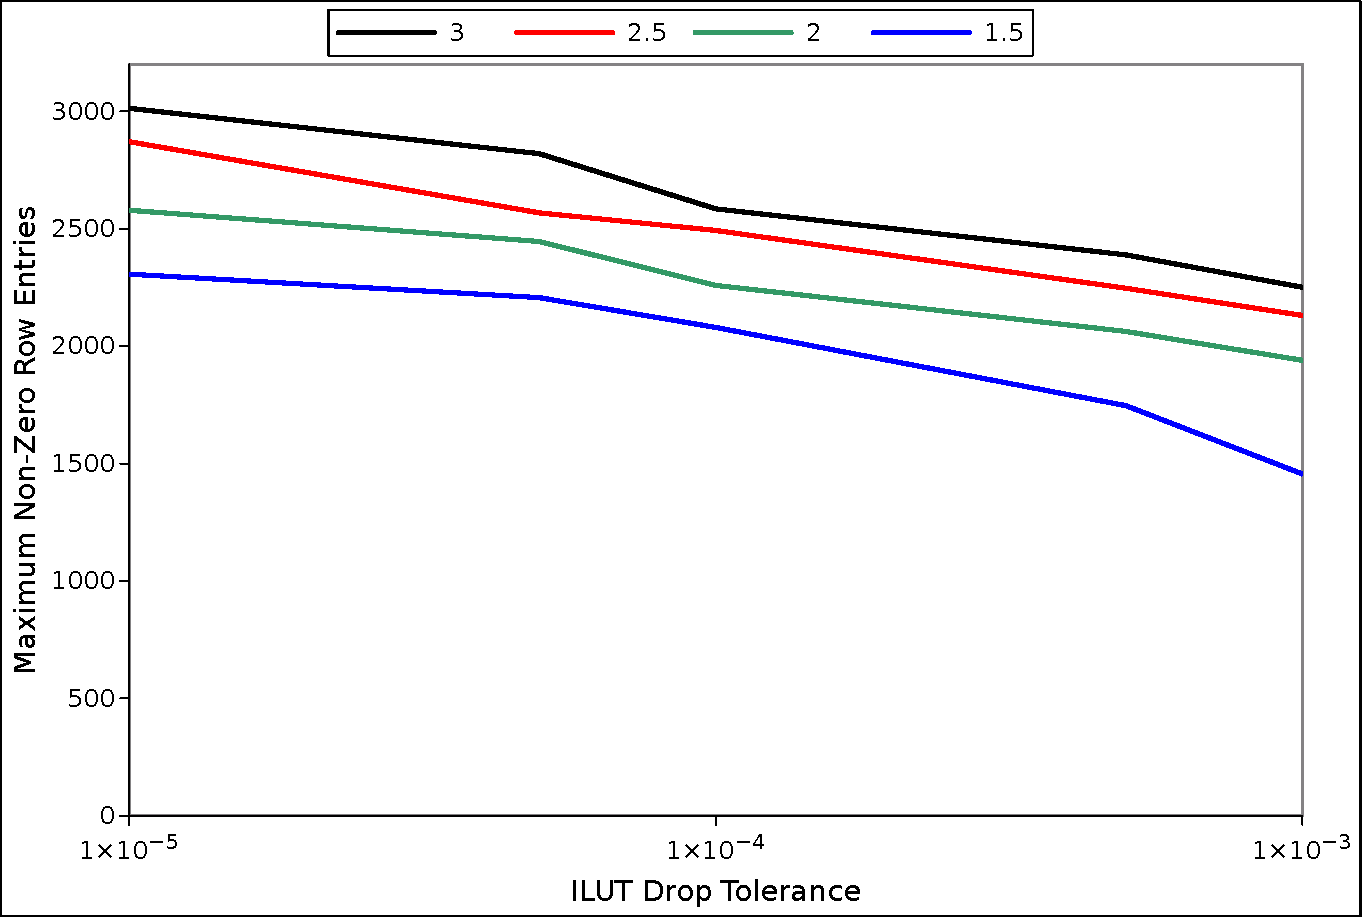
\includegraphics[width=4.25in]{chapters/spn_equations/ilut_size.pdf}
  \end{center}
  \caption{\textbf{Maximum number of non-zero entries observed for all
      rows in the composite linear operator for the fuel assembly
      problem with ILUT preconditioning given as a function of ILUT
      drop tolerance.} \textit{Each colored curve represents the row
      size for a different ILUT fill level. Fill levels of 1.5, 2.0,
      2.5, and 3.0 were used.}}
  \label{fig:ilut_size}
\end{figure}

As a means to assess the quality of the preconditioning, a simple
metric is developed to address these concerns and allow comparison to
future developments. For our studies, our core performance metric will
be iterative performance with the minimum number of MCSA iterations
required to converge the problem desired. For Monte Carlo
calculations, this improved performance is balanced by the creation of
a dense composite system and we seek to reduce the number of non-zero
entries to a minimum value in order to lower the amount of coupling
among states in the system and reduce the amount of memory used
along with the potential latency overhead. Given these two objectives,
the following metric is proposed:
\begin{equation}
  \text{Quality Metric} = (\text{\# iterations}) \times (\text{maximum
    \# non-zero values})\:,
\end{equation}
where the highest quality preconditioning is one that minimizes this
metric. For the ILUT preconditioned data provided,
Figure~\ref{fig:ilut_quality} provides the computed metric as a
function of ILUT drop tolerance for each fill level used. In general,
the metric is similar to the data observed for the number of
iterations required to converge as the non-zero row entries changed by
a smaller fraction over drop tolerances tested.
\begin{figure}[t!]
  \begin{center}
    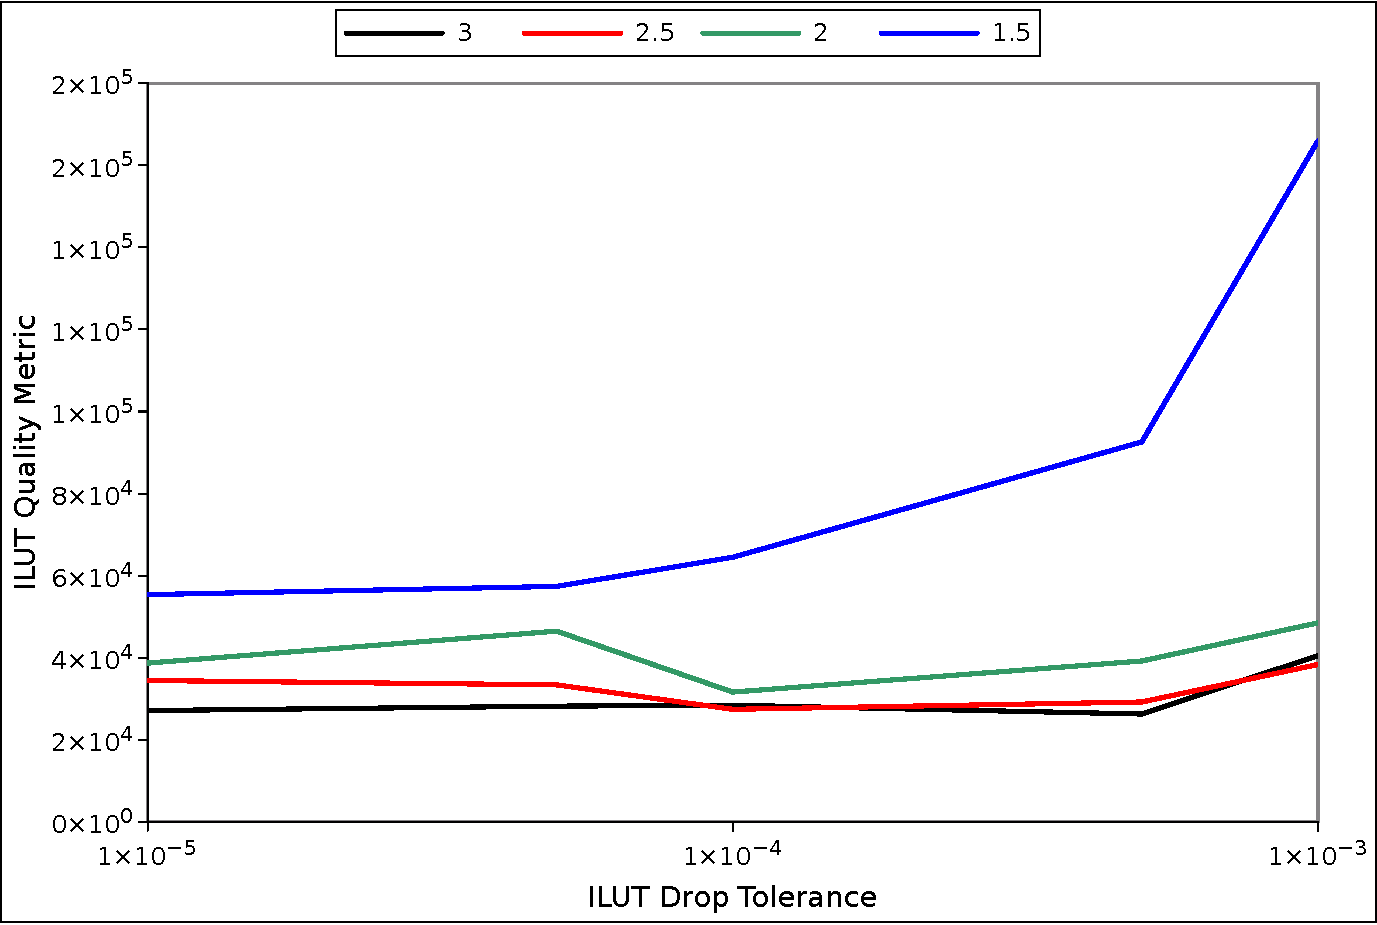
\includegraphics[width=4.25in]{chapters/spn_equations/ilut_quality.pdf}
  \end{center}
  \caption{\textbf{ILUT preconditioning quality metric for the fuel
      assembly problem given as a function of ILUT drop tolerance.}
    \textit{Each colored curve represents the quality metric behavior
      for a different ILUT fill level. Fill levels of 1.5, 2.0, 2.5,
      and 3.0 were used.}}
  \label{fig:ilut_quality}
\end{figure}

It should be noted here that although only the behavior of the linear
solve during a single eigenvalue iteration is reported, the behavior
of the linear solver was observed to be consistent throughout the
eigenvalue iterations (25 total eigenvalue iterations were required to
converge the 1-group $SP_1$ problem). We expect this as the linear
operator (which is unchanging in the fuel assembly criticality
problem) dictates the convergence of MCSA. At each iteration the
fission source provided to the linear problem is changing, however, we
expect the same convergence behavior for all source vectors
$\mathbf{b} \in \mathbb{R}^{N}$ where $||\mathbf{b}||_1 \neq 0$.

\subsection{Sparse Approximate Inverse Preconditioning}
\label{subsec:spn_spainv_preconditioning}
SPAINV is chosen because it the true inverse of the preconditioner is
byproduct of the algorithm and the algorithm seeks to maintain the
sparsity of the inverse preconditioner, potentially alleviating some
of the issues observed with ILUT. Explicit formation of the
preconditioner inverse is a requirement of the current MCSA
preconditioning strategy. As a result, although ILUT preconditioning
provided excellent iterative performance, a significant time penalty
is paid to extract the inverse of the triangular factors through $N$
triangular solves. In addition, this explicit inversion yielded a
composite linear operator that was dense, requiring modification of
the system in order to achieve better scalability and Monte Carlo
performance. Sparse approximate inverse (SPAINV) preconditioning is a
technique that may potentially alleviate both of these constraints at
the cost of reduced iterative performance. The method produces a
sparse approximation of the inverse matrix directly by minimizing the
Frobenius norm of the residual matrix \cite{saad_iterative_2003}:
\begin{equation}
  || \mathbf{I} - \mathbf{A} \mathbf{M} ||^2_F =
  \sum_{j=1}^N ||\mathbf{e}_j - \mathbf{A} \mathbf{m}_j||^2_2 \:,
  \label{eq:frobenius_norm_min}
\end{equation}
where the inverse preconditioning matrix $\mathbf{M}$ minimizes the
norm on the right and $\mathbf{e}_j$ and $\mathbf{m}_j$ are the
$j^{th}$ columns of the identity and preconditioning matrices
respectively. Here, $\mathbf{M}$ is the actual inverse of the
preconditioner and is formed directly by the algorithm. On the right
hand side of Eq~(\ref{eq:frobenius_norm_min}), the Frobenius norm is
represented as a effective sum of $N$ linear system residual norms. 

A few iterations of a subspace method or other iterative scheme can be
used to effectively solve these systems to a loose tolerance and yield
the columns of the approximate preconditioning matrix. At each
iteration, threshold values are used to eliminate the components of
each $\mathbf{m}_j$ column to maintain the desired level of
sparsity. In addition, a sparsity pattern can be predetermined and
enforced during this process. For the SPAINV implementation used for
this work, the sparsity pattern was defined by levels such that a
level of $N$ for an input operator $\mathbf{A}$ will generate a
preconditioning matrix $\mathbf{M}$ with the same sparsity pattern as
$\mathbf{A}^{N+1}$. By using the norm minimization strategy instead of
a factorization such as ILUT, parallel results are reproduced
regardless of parallel problem size, meaning that a serial computation
will converge in the same number of iterations as a computation with
thousands of cores.

MCSA preconditioned with SPAINV was used to solve the fuel assembly
problem as with ILUT for a 1-group $SP_1$ discretization. To study
convergence sensitivity to SPAINV parameters, the number of levels in
the sparsity pattern and threshold were parametrically varied with the
number of iterations to converge a single eigenvalue iteration for the
fuel assembly problem recorded along with the maximum number of
non-zero entries observed in all matrix rows for the preconditioned
composite linear operator. For each calculation, the number of
iterations required to converge reported was for a single eigenvalue
iteration with \sn{3}{4} histories at each MCSA iteration to compute
the Monte Carlo correction using the adjoint collision estimator. All
SPAINV calculations reported here were performed on a single CPU.

Figure~\ref{fig:spainv_iterations} gives the number of MCSA iterations
needed to converge the fuel assembly problem and
Figure~\ref{fig:spainv_size} the maximum number of non-zero entries
per row observed in the composite linear operator as a function the
SPAINV threshold. For this analysis, the number of levels in the
sparsity pattern was varied from 3 to 7 with convergence of the fuel
assembly problem not achieved for smaller level values. Compared to
ILUT preconditioning, at higher levels we see comparable iterative
performance with a relative invariance to the threshold value. The
threshold did have a significant effect, however, on the time required
to generate the preconditioner with a threshold of 0.001 over an order
of magnitude slower than a threshold of 0.01 due to the inclusion of a
significant number of extra values in the input operator. In addition
to comparable iterative performance, the sparsity of the composite
operator is greatly improved with nearly an order of magnitude
reduction in number of non-zero entries per row for lower level
values.
\begin{figure}[t!]
  \begin{center}
    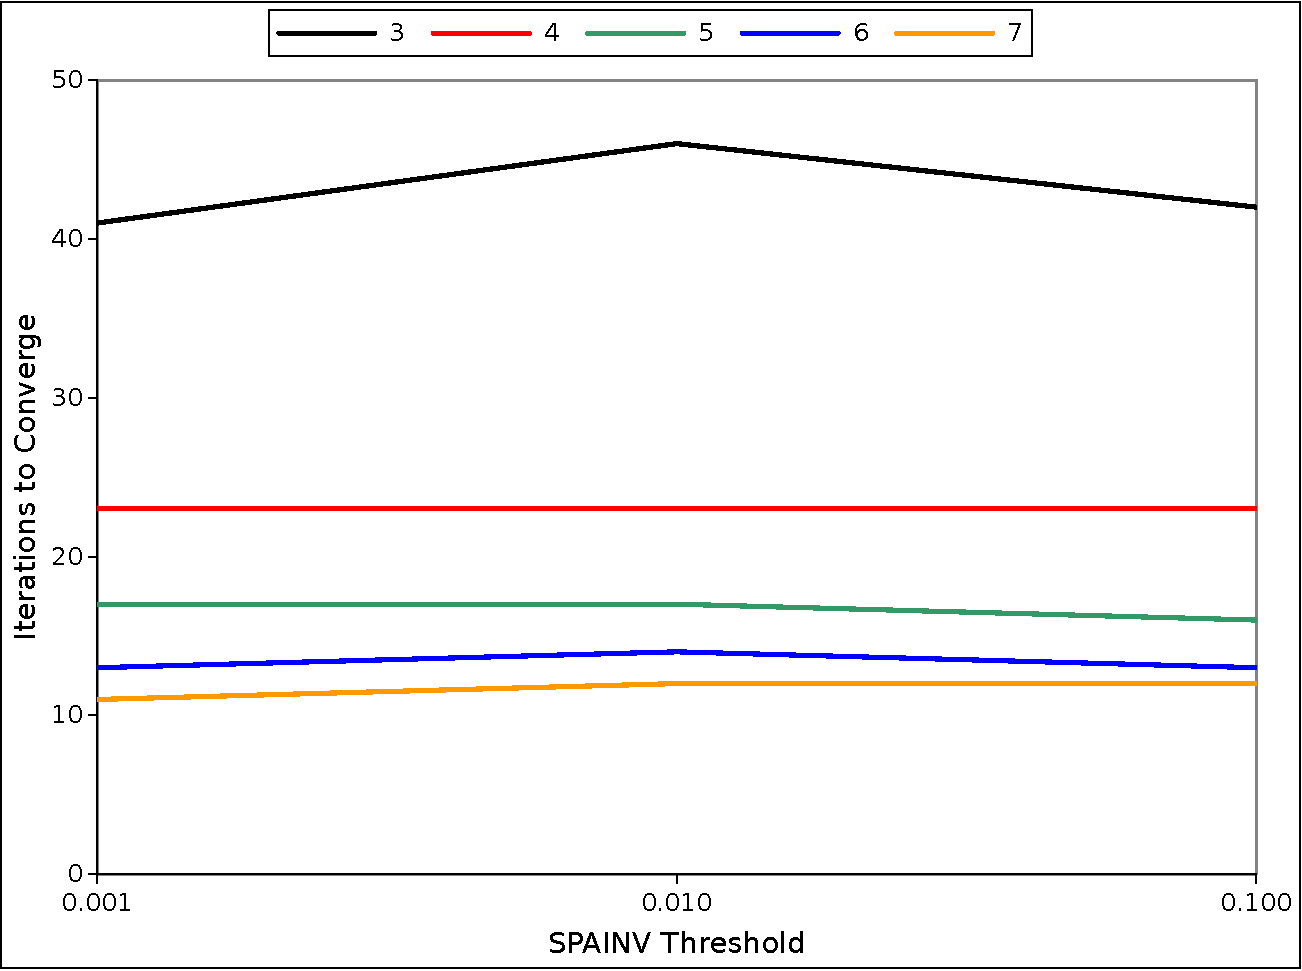
\includegraphics[width=4.25in]{chapters/spn_equations/spainv_iterations.pdf}
  \end{center}
  \caption{\textbf{Number of MCSA iterations required to converge a
      single eigenvalue iteration for the fuel assembly problem with
      SPAINV preconditioning as a function of SPAINV threshold.}
    \textit{Each colored curve represents the iteration behavior for a
      different SPAINV level pattern. Levels of 3, 4, 5, 6, and 7 were
      used.}}
  \label{fig:spainv_iterations}
\end{figure}
\begin{figure}[t!]
  \begin{center}
    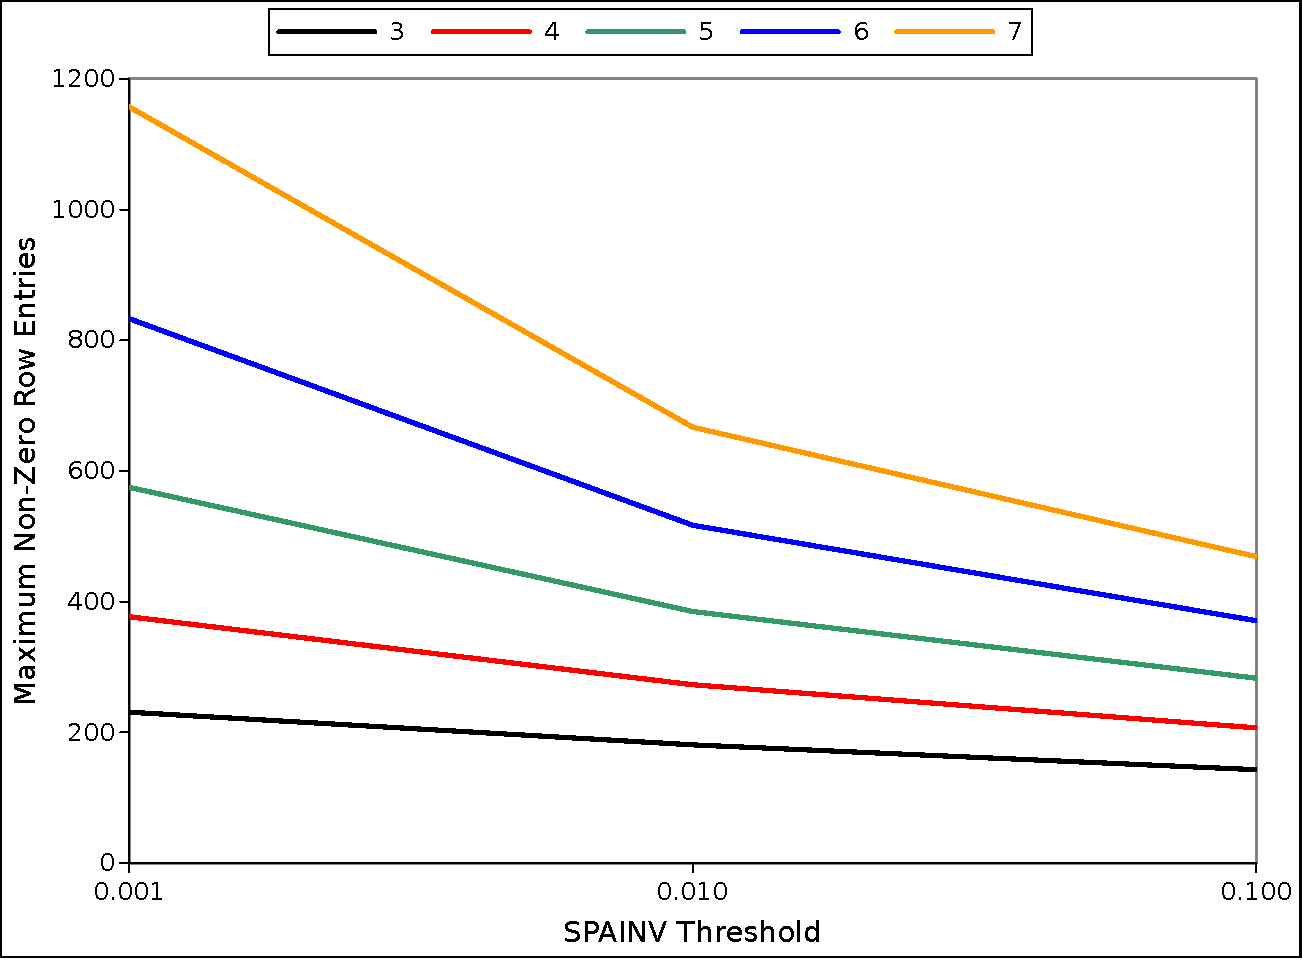
\includegraphics[width=4.25in]{chapters/spn_equations/spainv_size.pdf}
  \end{center}
  \caption{\textbf{Maximum number of non-zero entries observed for all
      rows in the composite linear operator for the fuel assembly
      problem with SPAINV preconditioning given as a function of
      SPAINV threshold.} \textit{Each colored curve represents the row
      size for a different SPAINV level pattern. Levels of 3, 4, 5, 6,
      and 7 were used.}}
  \label{fig:spainv_size}
\end{figure}

With the comparable iterative performance and improved sparsity,
SPAINV preconditioning should then have a more favorable quality
metric than ILUT preconditioning. Figure~\ref{fig:spainv_quality}
gives the quality metric as a function of the threshold value for each
of the sparsity levels computed. Not only do we see an improved
quality metric over ILUT preconditioning (about an order of magnitude
less), but we also note that the ideal sparsity level is not the largest
nor the smallest. In fact, the largest and smallest levels (3 and 7)
performed the worst in terms of the quality metric with a level of 4
performing the best. When CPU time to generate the preconditioner is
considered, 4 is the clear choice for this problem as more time is
required to do the approximate inversion as the sparsity pattern of
the preconditioner grows in size.
\begin{figure}[t!]
  \begin{center}
    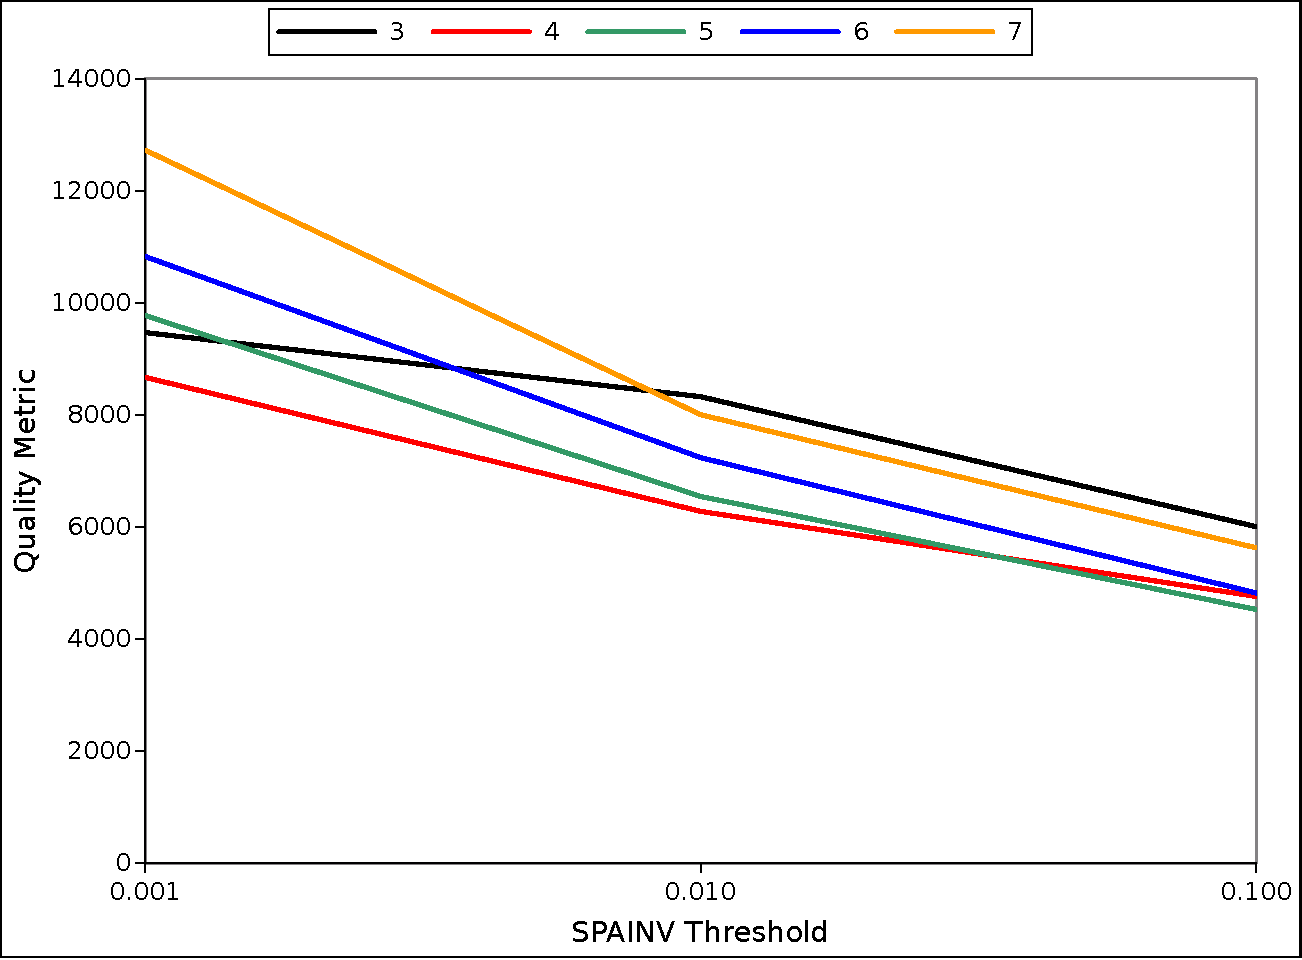
\includegraphics[width=4.25in]{chapters/spn_equations/spainv_quality.pdf}
  \end{center}
  \caption{\textbf{SPAINV preconditioning quality metric for the fuel
      assembly problem given as a function of SPAINV threshold.}
    \textit{Each colored curve represents the quality metric behavior
      for a different SPAINV level pattern. Levels of 3, 4, 5, 6, and
      7 were used.}}
  \label{fig:spainv_quality}
\end{figure}

\clearpage

\subsection{Applying the Reduced Domain Approximation}
\label{subsec:spn_prec_rda}
For each preconditioning technique presented convergence was achieved
for the single fuel assembly problem. However, a primary concern is
the number of non-zero states in each row of the system generated by
the explicit preconditioning strategy. In many cases, orders of
magnitude more matrix elements were generated resulting in poor
scalability for domain decomposed algorithms and overall performance
issues for Monte Carlo. As outlined in
\S~\ref{subsec:reduced_domain_approximation}, the reduced domain
approximation may be used as a mechanism to potentially alleviate this
problem by filtering elements of the composite matrix in each row that
fall below a certain threshold value or by maintaining the largest $N$
elements in each row where $N$ is a designated fill level.

For the ILUT, SPAINV, and SPAINV-ILUT preconditioning strategies the
reduced domain approximation will be applied to reduce the density of
the composite linear operator to more manageable levels. For each
preconditioner, the parameters that achieved the best quality metric
results from the previous analysis were used. These correspond to ILUT
parameters of a fill level of 5.0 and a drop tolerance of \sn{1}{-5},
SPAINV parameters of a sparsity level of 4 and a threshold of 0.1 and
SPAINV-ILUT with ILUT parameters of a fill level of 4.0 and a drop
tolerance of \sn{1}{-5} and SPAINV parameters of a sparsity level of 1
and a threshold of 1.0. The reduced domain threshold was set to
\sn{1}{-10} in order to eliminate any exceedingly small values from
the matrix (often this is simply removing non-zero elements within the
floating point tolerance of zero). The reduced domain fill level was
then varied, starting with the largest non-zero entries per row value
observed for each of the preconditioning types in order to assess its
effects relative to the case where no reduced domain approximation was
applied.

Figure~\ref{fig:rda_iterations} gives the number of iterations
required to converge for each preconditioner type as a function of
reduced domain fill level. Figure~\ref{fig:rda_quality} gives the
corresponding quality metric for each data point where the number of
non-zero entries used to compute the metric is equivalent to the
reduced domain fill level. We first note that SPAINV preconditioning
alone is significantly more sensitive to the reduction in domain size
over the ILUT-based methods, although the preconditioner was of
$O(100)$ non-zero entries per row without any approximation
applied. For the ILUT-based methods, performance was significantly
better with convergence achieved in less than 40 MCSA iterations with
only 10 non-zero entries in each row (vs. 7 non-zero entries for the
case with no preconditioning). SPAINV-ILUT iterative performance was
marginally better than ILUT alone for all reduced domain fill
levels. However, it should be noted that the ILUT level of fill used
for the ILUT only calculations was set to 4 for this case while the
SPAINV-ILUT preconditioner used an ILUT level of fill of 5 and
therefore the marginally better performance is more likely a result of
this addition of fill rather than the extra SPAINV
preconditioning. Looking at the quality metric data, we see a
reduction in the quality metric as a function of the reduced domain
fill level, achieving 2 orders of magnitude reduction in the quality
metric for the ILUT-based preconditioning methods.

Although applying the reduced domain approximation results in a
successful recovery of sparsity for the Monte Carlo problem while
maintaining good convergence properties, there is still an issue of
forming the composite operator before applying the approximation and
potentially generating the transpose of this operator in the case of
the adjoint Monte Carlo method. Because of this, memory and scaling
issues may still be observed when building the probability and weight
matrices for the Monte Carlo problem. In addition, the expensive
extraction of the inverse of the preconditioning operators for the
explicit scheme creates a significant cost in overall
performance. Future work in this area should be considerate of these
important components of the preconditioned MCSA algorithm.

\begin{figure}[t!]
  \begin{center}
    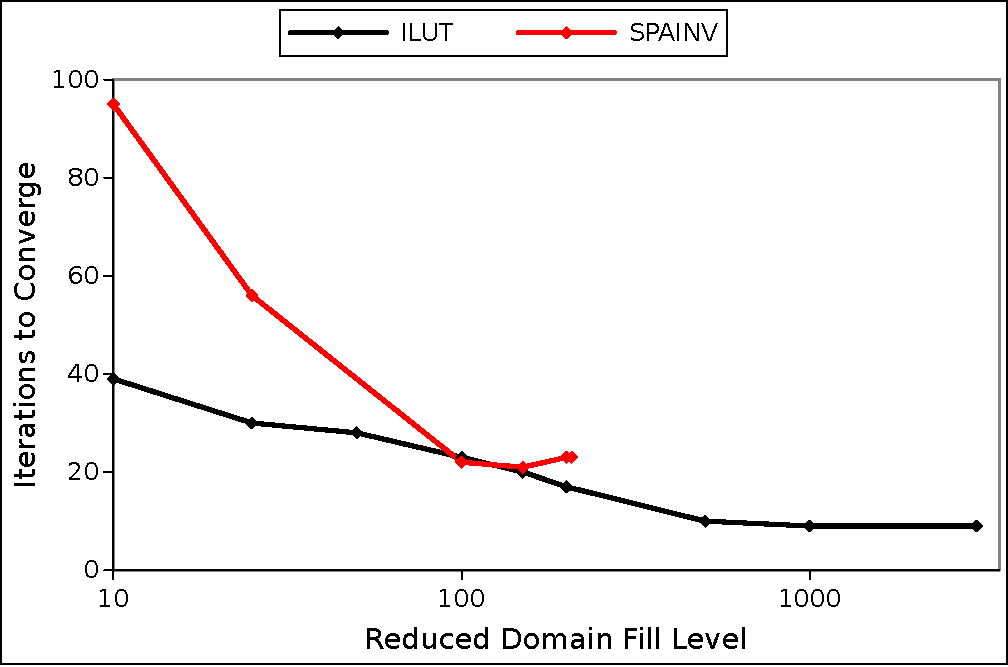
\includegraphics[width=4.25in]{chapters/spn_equations/rda_iterations.pdf}
  \end{center}
  \caption{\textbf{Number of MCSA iterations required to converge a
      single eigenvalue iteration for the fuel assembly problem with
      each preconditioning as a function of reduced domain
      approximation fill level.} \textit{The largest fill level for
      each preconditioning presented is that using the parameters that
      gave the best results without the approximation.}}
  \label{fig:rda_iterations}
\end{figure}

\begin{figure}[t!]
  \begin{center}
    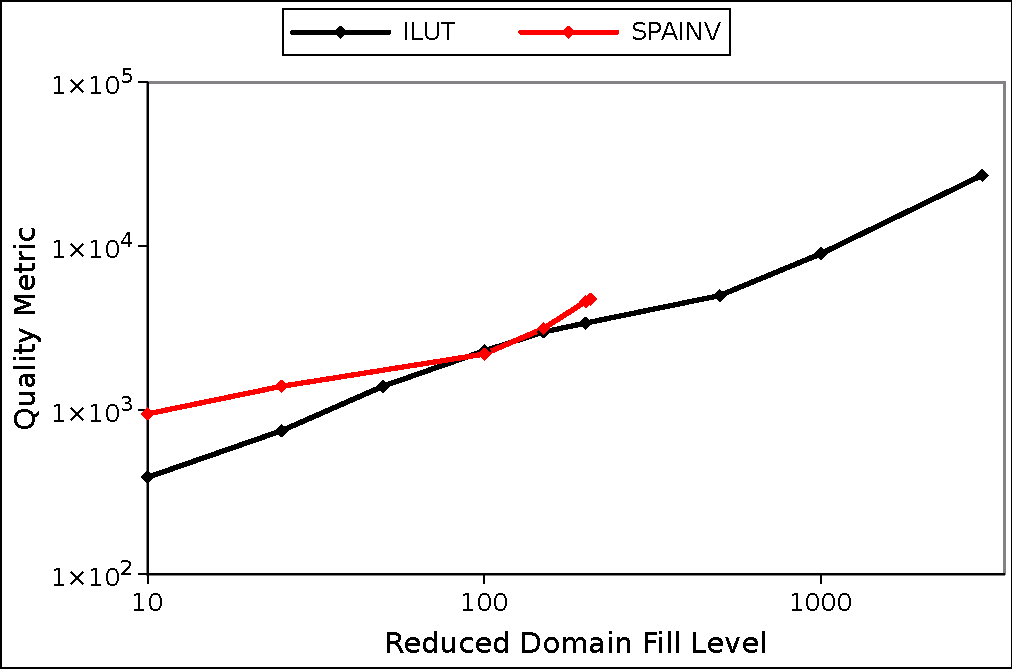
\includegraphics[width=4.25in]{chapters/spn_equations/rda_quality.pdf}
  \end{center}
  \caption{\textbf{Preconditioning quality metric for the fuel
      assembly problem given as a function of reduced domain
      approximation fill level.} \textit{The largest fill level for
      each preconditioning presented is that using the parameters that
      gave the best results without the approximation.}}
  \label{fig:rda_quality}
\end{figure}

\clearpage

\subsection{MCSA Relaxation Parameters}
\label{subsec:spn_mcsa_relaxation}
As another means of preconditioning (or variance reduction) to meet
the goal of improving iterative performance, the Richardson iteration
upon which the Neumann-Ulam method is built may be implemented with an
adjustable scalar relaxation parameter:
\begin{equation}
  \mathbf{x} = \mathbf{x} + \omega \mathbf{r}\:,
  \label{eq:richardson_relaxation}
\end{equation}
where $\omega$ is the relaxation parameter. This is very similar to
point Jacobi preconditioning where the system is now being scaled on
the left by a constant value in all rows. Analogously, these
relaxation parameter techniques can be applied to Monte Carlo to
improve convergence as demonstrated by Dimov \cite{dimov_new_1998}. In
this case, building an iteration matrix from
Eq~(\ref{eq:richardson_relaxation}) gives:
\begin{equation}
  \mathbf{H} = \mathbf{I} - \omega \mathbf{A}\:,
  \label{eq:relaxed_iteration_matrix}
\end{equation}
with the probabilities and weights for the Monte Carlo procedure
appropriately scaled via a modified Neumann-Ulam decomposition. For
MCSA, we can stage this scheme with two separate relaxation
parameters; one for the outer Richardson iteration and one for the
inner Monte Carlo solve:
\begin{subequations}
  \begin{gather}
    \ve{x}^{k+1/2} = \ve{x}^k + \omega_R \ve{r}^k\:,\\ \ve{r}^{k+1/2}
    = \ve{b} -
    \ve{A}\ve{x}^{k+1/2}\:,\\ \omega_N\ve{A}\delta\ve{x}^{k+1/2} =
    \omega_N\ve{r}^{k+1/2}\:,\\ \ve{x}^{k+1} = \ve{x}^{k+1/2} + \delta
    \ve{x}^{k+1/2}\:,\\ \ve{r}^{k+1} = \ve{b} - \ve{A}\ve{x}^{k+1}\:,
  \end{gather}
  \label{eq:mcsa_relaxed}
\end{subequations}
where $\omega_R$ is the Richardson iteration relaxation parameter and
$\omega_N$ is the Neumann-Ulam Monte Carlo solve relaxation parameter.

We apply these relaxation parameters to the fuel assembly problem
along with the reduced domain approximation as a means of studying
their effects. For each calculation presented, the number of
iterations required to converge reported was for a single eigenvalue
iteration.  Again, \sn{3}{4} histories are used at each MCSA iteration
to compute the Monte Carlo correction using the adjoint collision
estimator. A reduced domain fill level of 100 is used with a threshold
of \sn{1}{-10} to filter small values. ILUT preconditioning with a
drop tolerance of \sn{1}{-5} and fill level of 5 is used as
well. 

Figure~\ref{fig:relax_iters} gives the number of iterations required
to converge the fuel assembly problem for a 1-group SP1 discretization
using varying combinations of the relaxation parameters. First, both
parameters were fixed at the base case of 1 while the other parameter
was varied as shown in the left-hand side plots of
Figure~\ref{fig:relax_iters}. For the Richardson relaxation parameter,
using a value larger than 1 gave better iterative performance up to a
point, effectively providing a stronger extrapolation using the
residual at each iteration. For the Neumann relaxation parameter, a
value of less than 1 is observed to be ideal. Although initially
counter-intuitive, the fact that the correction computed by the Monte
Carlo solver has a stochastic error associated with it means that by
using a Neumann relaxation parameter less than 1, the correction and
its error are effectively dampened to improve iterative
performance. Considering the CPU time required to converge a single
eigenvalue iteration, similar results are also observed for the
relaxation parameters as given by Figure~\ref{fig:relax_time}. For the
base cases given by the plots on the left, it was found the a
Richardson relaxation parameter of 1.1 and a Neumann relaxation
parameter of 0.7 provided the fastest CPU time for convergence. Fixing
each parameter at these new values, the calculations were repeated as
shown for the plots on the right hand sides of both
Figures~\ref{fig:relax_iters} and \ref{fig:relax_time}. For each
repeated timing calculation, it was found that the same combination of
relaxation parameters found in the base cases performed the best
although they did not necessarily have the best iterative performance.

\begin{figure}[t!]
  \begin{center}
    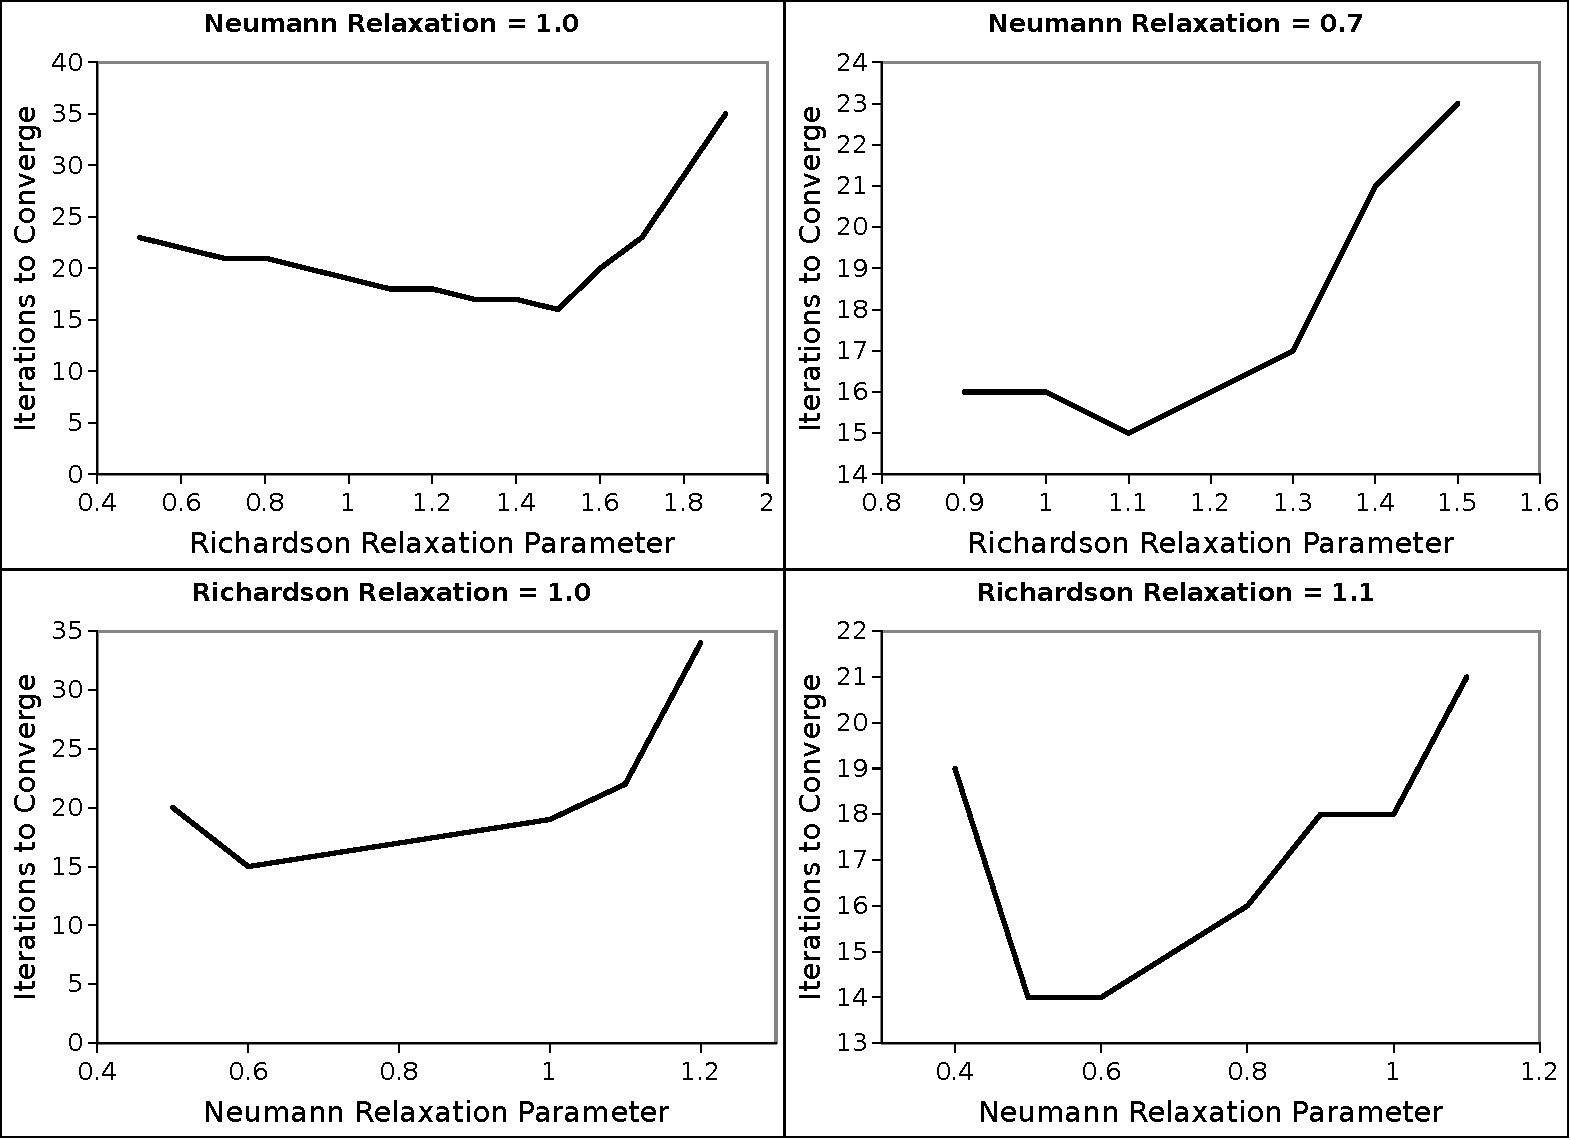
\includegraphics[width=6in]{chapters/spn_equations/relax_iters.pdf}
  \end{center}
  \caption{\textbf{Number of iterations to converge a single
      eigenvalue iteration of the fuel assembly problem as a function
      of the relaxation parameters.} \textit{Starting in upper left
      and moving counter-clockwise: Neumann relaxation parameter fixed
      at 1.0, Richardson relaxation parameter fixed at 1.0, Neumann
      relaxation parameter fixed at 0.7, Richardson relaxation
      parameter fixed at 1.1. For each calculation \sn{3}{4}
      stochastic histories were used to compute the MCSA correction at
      each iteration.}}
  \label{fig:relax_iters}
\end{figure}

\begin{figure}[t!]
  \begin{center}
    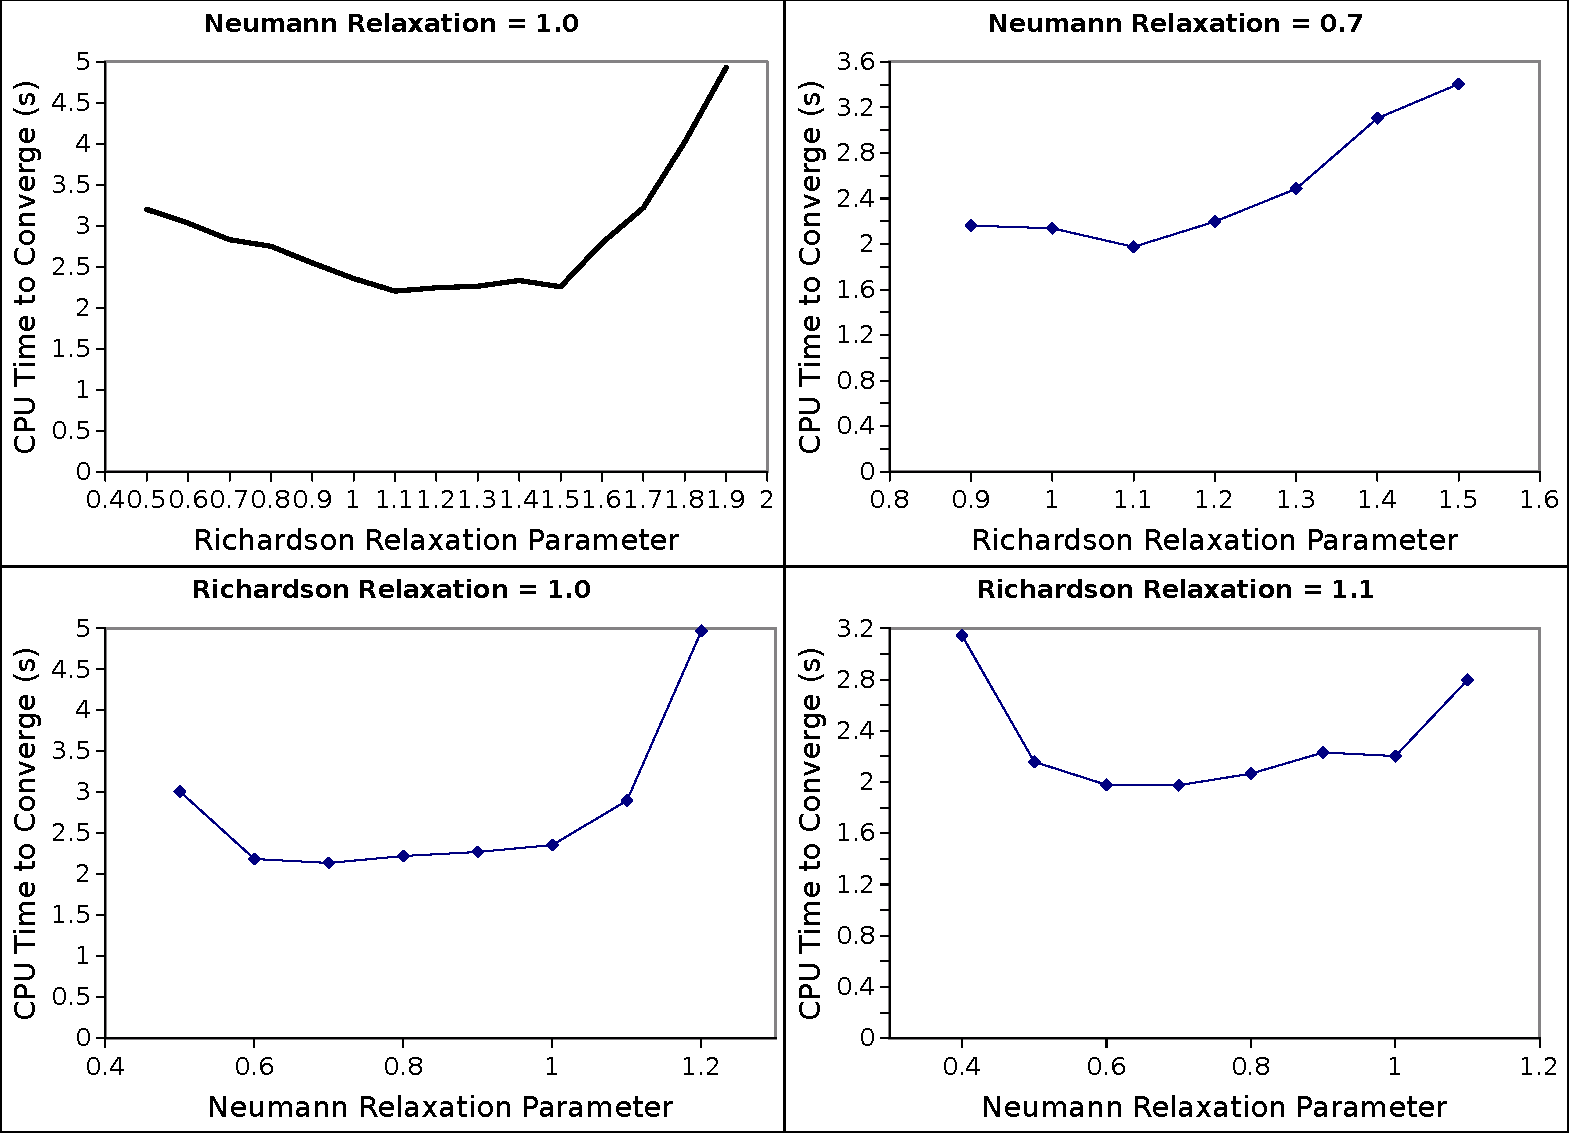
\includegraphics[width=6in]{chapters/spn_equations/relax_time.pdf}
  \end{center}
  \caption{\textbf{CPU time in seconds to converge a single eigenvalue
      iteration of the fuel assembly problem as a function of the
      relaxation parameters.} \textit{Starting in upper left and
      moving counter-clockwise: Neumann relaxation parameter fixed at
      1.0, Richardson relaxation parameter fixed at 1.0, Neumann
      relaxation parameter fixed at 0.7, Richardson relaxation
      parameter fixed at 1.1. For each calculation \sn{3}{4}
      stochastic histories were used to compute the MCSA correction at
      each iteration.}}
  \label{fig:relax_time}
\end{figure}

\clearpage

\subsection{MCSA Estimator and Fixed Point Iteration Analysis}
\label{subsec:spn_estimator_comparison}
With convergence obtained for the fuel assembly problem, the iterative
performance of MCSA will next be studied with both the collision and
expected value estimators using the best preconditioning and
relaxation parameter combinations found by the previous
analysis. Additionally, both the Richardson-based MCSA iteration given
by Eq~(\ref{eq:mcsa}) and the minimal residual-based MCSA iteration
given by Eq~(\ref{eq:mcsa_min_res}) will be used. Although the
expected value estimator achieved the best iterative performance in
the previous comparison and analysis for the simple Poisson problem in
\S~\ref{sec:parameter_estimator_analysis}, it is possible that the
collision estimator may perform better from a timing perspective due
to the sparsity lost by explicit preconditioning. The deterministic
component of the expected value estimator that couples the current
state to other local states through the iteration matrix stencil
requires application of the estimator to potentially several orders of
magnitude more states at every transition event.

For this study, the fuel assembly problem with a 1-group $SP_1$
discretization was solved using MCSA with the adjoint Monte Carlo
solver using both the collision and expected value estimators and both
the Richardson and minimal residual fixed point iterations. Using the
results from the previous section, a Neumann relaxation parameter of
0.7 was used with both estimators and fixed point iterations. For the
collision estimator, a Richardson relaxation parameter of 1.1 was used
with the Richardson iteration while it was found the expected value
estimator had the best performance when a Richardson relaxation
parameter of 1.0 was used instead. In addition, ILUT preconditioning
with a drop tolerance of \sn{1}{-5} and a fill level of 5 was used
with a reduced domain approximation fill level of 100 and a threshold
of \sn{1}{-10} as in the previous analysis. Artificial absorption was
also introduced with a value of 0.2 for the MCSA calculations that
used the collision estimator as CPU timing performance was improved
without a loss in iterative performance while no absorption was used
for calculations using the expected value estimator. For each
estimator, the number of stochastic histories used to compute the MCSA
correction was varied from 25 to 50,000 with the number of MCSA
iterations required to converge to a tolerance of \sn{1}{-8} recorded
for a single eigenvalue iteration along with the CPU time required to
achieve convergence.

Figure~\ref{fig:spn_estimator_iters} gives the iteration count results
and Figure~\ref{fig:spn_estimator_time} gives the timing
results. Remarkably, although the fuel assembly problem is
significantly more complicated than the simple Poisson problem studied
in \S~\ref{sec:parameter_estimator_analysis}, the results here are
largely the same with Figure~\ref{fig:spn_estimator_iters} and
Figure~\ref{fig:estimator_nh_iters} having identical qualitative
behavior. Using the expected value estimator with both fixed point
iterations again creates a relative insensitivity to the number of
histories used to compute the correction. Marginally better iterative
and timing performance was observed for the expected value estimator
when using the Richardson iteration. Better timing performance is
expected as computing the extrapolation parameter in the minimal
residual iteration requires several additional parallel
operations. Compared to the collision estimator, the minimal residual
iteration permits fewer stochastic histories to be used with each MCSA
iteration while still maintaining good iterative performance. With
respect to CPU time, there is a more pronounced effect due to the
larger density of states created by the explicit ILUT
preconditioning. Using a reduced domain fill level of 100 creates a
situation where the expected value estimator is significantly more
expensive per history to compute that the collision estimator due to
the coupling of states.

\begin{figure}[t!]
  \begin{center}
    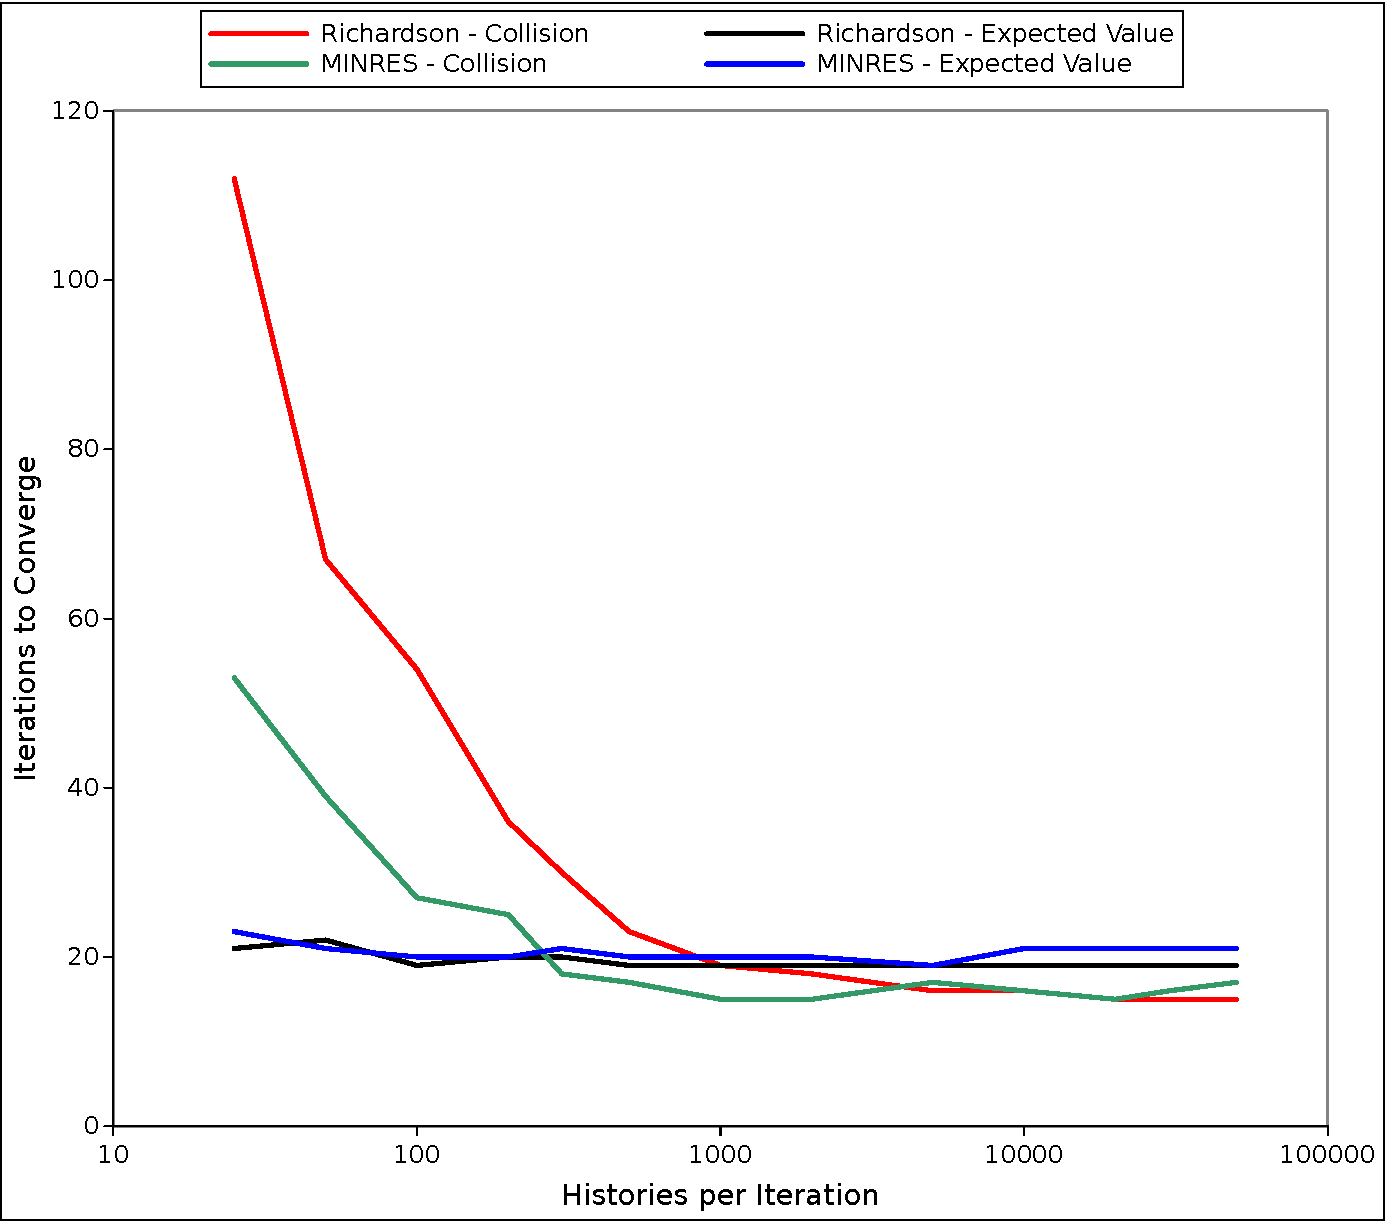
\includegraphics[width=5in]{chapters/spn_equations/estimator_iters.pdf}
  \end{center}
  \caption{\textbf{MCSA iterations required to converge the fuel
      assembly problem to a tolerance of \sn{1}{-8}.} \textit{Both the
      collision and expected value estimators were used with the
      adjoint Monte Carlo solver to compute the correction at each
      iteration. Each estimator was used with the Richardson and
      minimal residual fixed point iterations within an MCSA
      iteration.}}
  \label{fig:spn_estimator_iters}
\end{figure}

\begin{figure}[t!]
  \begin{center}
    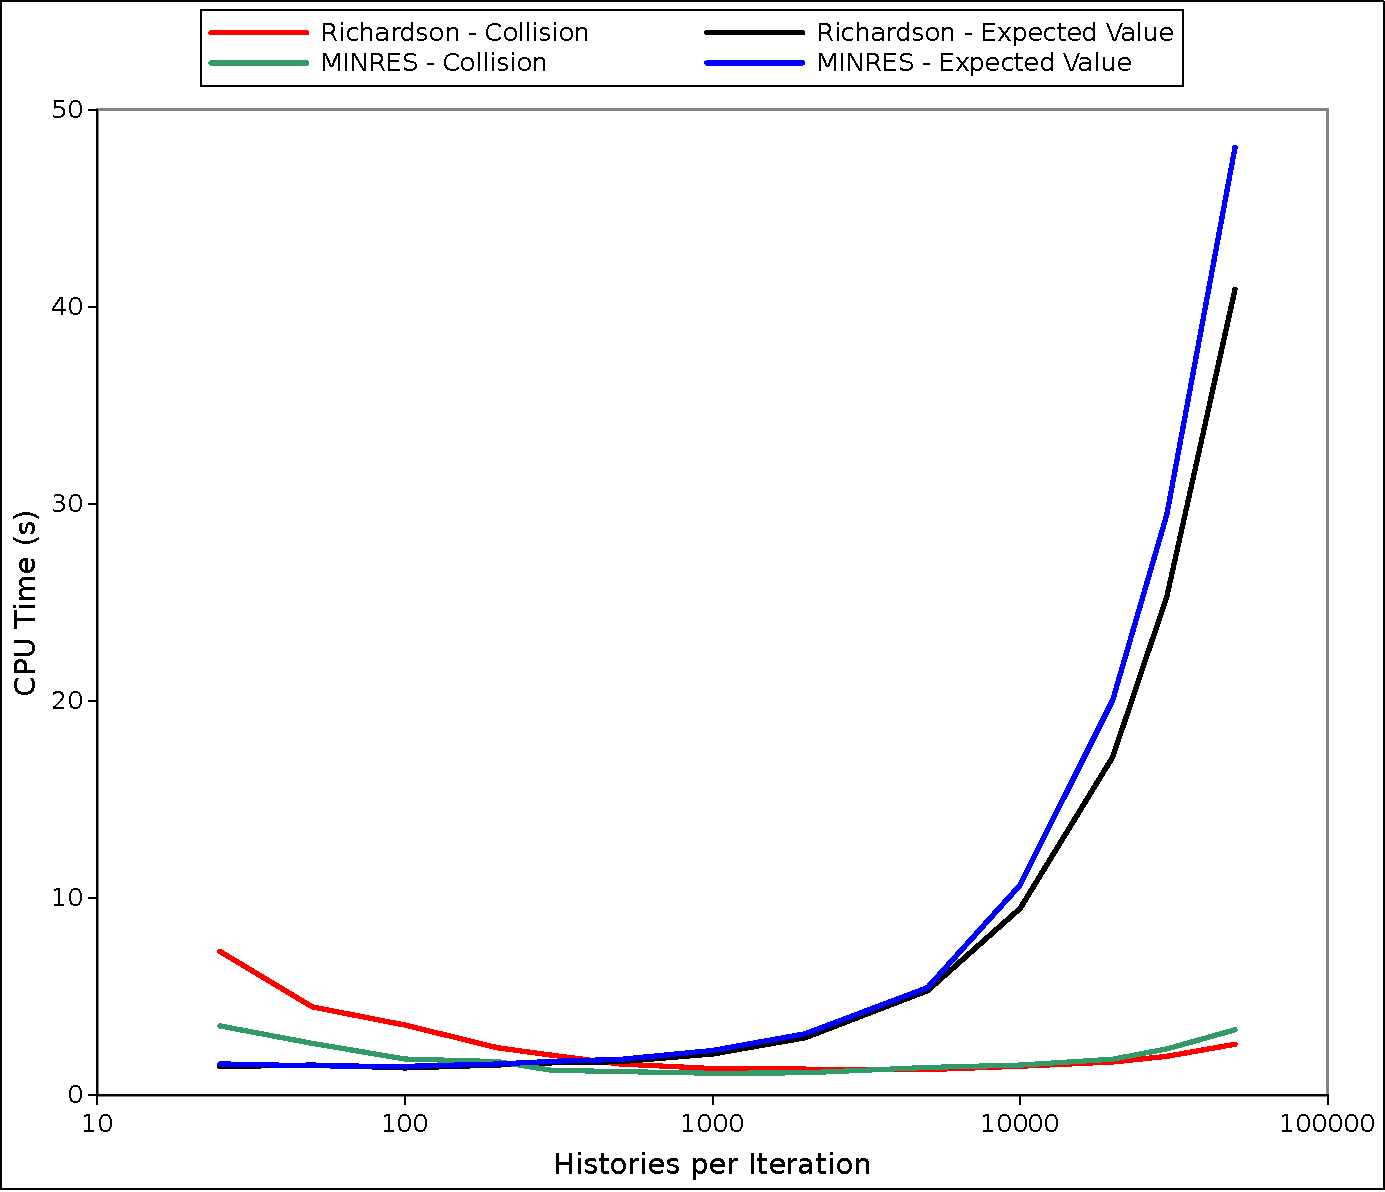
\includegraphics[width=5in]{chapters/spn_equations/estimator_time.pdf}
  \end{center}
  \caption{\textbf{Total CPU time in seconds required to converge the
      fuel assembly problem to a tolerance of \sn{1}{-8}.}
    \textit{Both the collision and expected value estimators were used
      with the adjoint Monte Carlo solver to compute the correction at
      each iteration. Each estimator was used with the Richardson and
      minimal residual fixed point iterations within an MCSA
      iteration.}}
  \label{fig:spn_estimator_time}
\end{figure}

From both Figure~\ref{fig:spn_estimator_iters} and
Figure~\ref{fig:spn_estimator_time} we see that both estimators and
fixed point iterations have comparable iterative and timing
performance when 1,000 histories are used at each MCSA
iteration. Using 1,000 histories per MCSA iteration, the infinity norm
of the residual vector is presented at every MCSA iteration for both
estimators and both fixed point iterations in
Figure~\ref{fig:spn_estimator_convergence} as an additional means of
comparison. At this number of histories, all MCSA combinations
converge the fuel assembly problem monotonically at approximately the
same rate, giving little reason to choose one over the other. The end
result is that both estimators provide a viable method for getting
good MCSA iterative performance with comparable timing
performance. For the collision estimator, using around 20,000
stochastic histories at every iteration gave the best iterative
performance while 500 histories per iteration gave the best iterative
performance when using the expected value estimator. For purely serial
computational performance, there is not a distinguishing feature for
the fuel assembly problem presented that would cause one to choose one
of the estimators and fixed point iterations over the other as they
all have similar minimum CPU times over the range of values tested.

\begin{figure}[t!]
  \begin{center}
    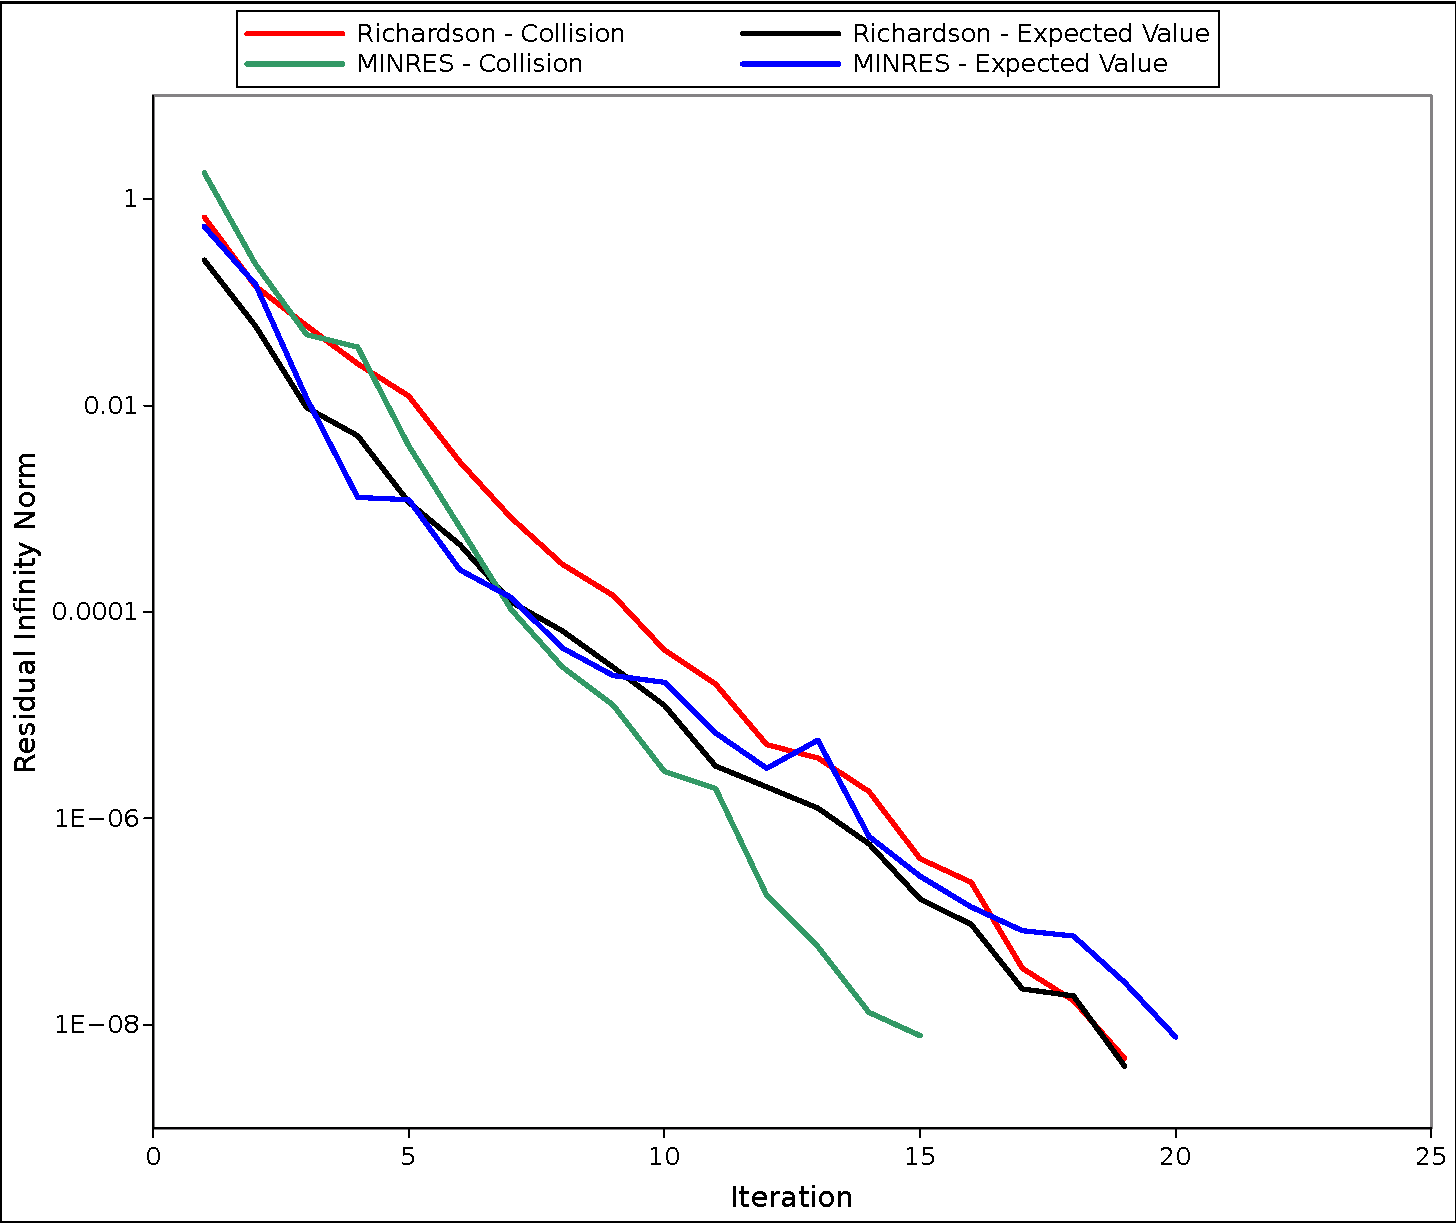
\includegraphics[width=5in]{chapters/spn_equations/estimator_convergence.pdf}
  \end{center}
  \caption{\textbf{Residual infinity norm as a function of MCSA
      iteration with 1,000 stochastic histories per iteration.}
    \textit{Both the collision and expected value estimators were used
      with the adjoint Monte Carlo solver to compute the correction at
      each iteration. Each estimator was used with the Richardson and
      minimal residual fixed point iterations within an MCSA
      iteration.}}
  \label{fig:spn_estimator_convergence}
\end{figure}

\clearpage

%%---------------------------------------------------------------------------%%
\section{MCSA Verification\ }
\label{sec:spn_mcsa_verification}
Through the numerical studies presented in this chapter, we have
developed a set of preconditioning techniques that permit MCSA to be
used with the $SP_N$ form of the neutron transport equation and
applied to a difficult fuel assembly criticality problem. Along with
these preconditioning techniques, a set a varying MCSA parameters were
analyzed to find those that yielded the best performance for this
particular problem. In addition, several steps were taken to mitigate
the dense composite linear operators that arise when performing
explicit MCSA preconditioning necessary for achieve convergence. Using
these results, we know compare MCSA directly to conventional linear
solvers that would be typically used to solve the $SP_N$ form of the
transport equation as presented here. In particular, we will use a
pair of Krylov solvers with which we will compare numerical results to
verify MCSA solutions the implementation used for this work.

MCSA solutions to the fuel assembly problem with 1, 2, and 4 energy
groups using $SP_1$ discretization will computed using both BiCGStab
and GMRES implementations from the Trilinos scientific computing
library Aztec \cite{heroux_overview_2005}. The neutron fluxes, the
number of eigenvalue iterations required to converge the problem, and
the eigenvalue itself will be compared as a means of verification. For
the flux values, we will look at the 2-norm and infinity norm of the
relative difference vector between the reference case and the
comparison case in each energy group:
\begin{equation}
  \text{Relative Group Flux Difference} = \frac{\ve{\Phi}_{ref}^g -
    \ve{\Phi}^g}{\ve{\Phi}_{ref}^g}\:,
  \label{eq:relative_difference_vector}
\end{equation}
where the addition and subtraction operations are performed
element-wise to construct the vector. For this work, the BiCGStab
results will be taken as the reference case.

All solvers will be preconditioned with ILUT using a drop tolerance of
\sn{1}{-5} and a fill level of 5. For GMRES, no restrictions were
placed on the size of the subspace and therefore no restarts
occurred. When the collision estimator was used with MCSA, \sn{2}{4}
stochastic histories were used to compute the correction for every
energy group in the problem (\sn{4}{4} and \sn{8}{4} histories total
for the 2 and 4 group calculations respectively) corresponding to
approximately 1 stochastic history per DOF. When the expected value
estimator was used, \sn{5}{2} stochastic histories used for each
energy group (\sn{1}{3} and \sn{1.5}{3} histories total for the 2 and
4 group calculations) giving approximately 1 stochastic history for
every 5 DOFs. The reduced domain approximation was also applied in
conjunction with the ILUT preconditioning using a fill level of 100
and a threshold value of \sn{1}{-10} to reduce the density of states
in the Monte Carlo problem. For relaxation parameters, all MCSA
computations used a Neumann relaxation parameter of 0.7 while a
Richardson relaxation of 1.1 was used with the collision estimator and
1.0 with the expected value estimator as determined by the previous
analysis. Table~\ref{tab:spn_solver_defs} gives definitions for the
solvers used to generate the results in the remainder of this
section. For the energy group structures,
Table~\ref{tab:spn_group_structure} gives the lower bounds of each
group in eV (an implicit upper bound of \sn{2}{6} eV is assumed for
group 0).
\begin{table}[h!]
  \begin{center}
    \begin{tabular}{ll}\hline\hline
      \multicolumn{1}{l}{\textbf{Name}} & 
      \multicolumn{1}{l}{\textbf{Definition}} \\
      BiCGStab-ILUT & BiCGStab preconditioned with ILUT \\
      GMRES-ILUT & GMRES preconditioned with ILUT \\
      MCSA-ILUT-R-C & MCSA preconditioned with ILUT using Richardson \\ 
                    & fixed point iteration and collision estimator \\
      MCSA-ILUT-MR-C & MCSA preconditioned with ILUT using minimal residual \\
                     & fixed point iteration and collision estimator \\
      MCSA-ILUT-R-EV & MCSA preconditioned with ILUT using Richardson \\
                     & fixed point iteration and expected value estimator \\
      MCSA-ILUT-MR-EV & MCSA preconditioned with ILUT using minimal residual \\
                      & fixed point iteration and expected value estimator \\
      Richardson-ILUT & Richardson iteration preconditioned with ILUT \\
      %%
      \hline\hline
    \end{tabular}
  \end{center}
  \caption{\textbf{Solver definitions used for MCSA verification and
      performance analysis.} \textit{The ILUT preconditioner
      parameters were identical for all calculations and solvers.}}
  \label{tab:spn_solver_defs}
\end{table}
\begin{table}[h!]
  \begin{center}
    \begin{tabular}{cl}\hline\hline
      \multicolumn{1}{c}{\textbf{Number of Groups}} & 
      \multicolumn{1}{l}{\textbf{Lower Bounds (eV)}} \\
      1 & \{ \sn{1}{-5} \} \\
      2 & \{ \sn{1}{-1}, \sn{1}{-5} \} \\
      4 & \{ \sn{1}{1}, \sn{1}{0}, \sn{1}{-1}, \sn{1}{-5} \} \\
      %%
      \hline\hline
    \end{tabular}
  \end{center}
  \caption{\textbf{Energy group lower bounds for the multigroup fuel
      assembly criticality problem in electron volts.} \textit{An
      implicit upper bound of \sn{2}{6} eV is assumed for group zero.}}
  \label{tab:spn_group_structure}
\end{table}

For every combination of energy group structure and solver, the
eigenvalue problem was converged with an eigensolver tolerance of
\sn{1}{-6} and a linear solver tolerance of \sn{1}{-8} in a serial
calculation. Table~\ref{tab:serial_ev_results} gives the eigenvalue
computed by each solver for each problem as well as the number of
eigenvalue iterations required to converge. For every problem, each
solver converged to the same eigenvalue up to the number of digits
reported by the eigensolver in the same number of eigenvalue
iterations.

\begin{table}[h!]
  \begin{center}
    \begin{tabular}{lccc}\hline\hline
      \multicolumn{1}{c}{\textbf{Solver}} & 
      \multicolumn{1}{c}{\textbf{Number of Groups}} & 
      \multicolumn{1}{c}{\textbf{Iterations}} &
      \multicolumn{1}{c}{\textbf{Eigenvalue}} \\
      \hline
      BiCGStab-ILUT & 1 & 25 & 1.105987 \\
      GMRES-ILUT & 1 & 25 & 1.105987 \\
      MCSA-ILUT-R-C & 1 & 25 & 1.105987 \\
      MCSA-ILUT-MR-C & 1 & 25 & 1.105987 \\
      MCSA-ILUT-R-EV & 1 & 25 & 1.105987 \\
      MCSA-ILUT-MR-EV & 1 & 25 & 1.105987 \\
      Richardson-ILUT & 1 & 25 & 1.105987 \\
      \hline
      BiCGStab-ILUT & 2 & 35 & 1.155239 \\
      GMRES-ILUT & 2 & 35 & 1.155239 \\
      MCSA-ILUT-R-C & 2 & 35 & 1.155239 \\
      MCSA-ILUT-MR-C & 2 & 35 & 1.155239 \\
      MCSA-ILUT-R-EV & 2 & 35 & 1.155239 \\
      MCSA-ILUT-MR-EV & 2 & 35 & 1.155239 \\
      Richardson-ILUT & 2 & 35 & 1.155239 \\
      \hline
      BiCGStab-ILUT & 4 & 31 & 1.175850 \\
      GMRES-ILUT & 4 & 31 & 1.175850 \\
      MCSA-ILUT-R-C & 4 & 31 & 1.175850 \\
      MCSA-ILUT-MR-C & 4 & 31 & 1.175850 \\
      MCSA-ILUT-R-EV & 4 & 31 & 1.175850 \\
      MCSA-ILUT-MR-EV & 4 & 31 & 1.175850 \\
      Richardson-ILUT & 4 & 31 & 1.175850 \\
      %%
      \hline\hline
    \end{tabular}
  \end{center}
  \caption{\textbf{Serial eigensolver verification results for the
      fuel assembly problem.} \textit{Each calculation was converged
      with the same eigensolver and linear solver
      tolerances. Table~\ref{tab:spn_solver_defs} gives the
      description for each solver type presented.}}
  \label{tab:serial_ev_results}
\end{table}

Table~\ref{tab:serial_differences_g1},
Table~\ref{tab:serial_differences_g2}, and
Table~\ref{tab:serial_differences_g4} give the infinity norms and
2-norms of the flux relative difference vectors given by
Eq~(\ref{eq:relative_difference_vector}) for all calculations and all
energy groups. In general, we see good agreement in the two norm
between the MCSA variants and the GMRES calculation, meaning that they
have approximately the same variation from the BiCGStab
calculation. We do note larger infinity norm values of this vector for
some of the MCSA variants (i.e. group 1 in the 2-group calculation),
however this large maximum value was not a global phenomenon with good
agreement in the 2-norm for the calculations. Based on the good
agreement between MCSA and GMRES for the relative difference of the
group fluxes and the eigenvalue results presented here, the MCSA
implementation should be deemed correct for the fuel assembly problem
for serial calculations with multiple energy groups.

\begin{table}[h!]
  \begin{center}
    \begin{tabular}{lccc}\hline\hline
      \multicolumn{1}{c}{\textbf{Solver}} & 
      \multicolumn{1}{c}{\textbf{Group}} &
      \multicolumn{1}{c}{\textbf{$|| \cdot ||_{inf}$}} &
      \multicolumn{1}{c}{\textbf{$|| \cdot ||_2$}} \\
      \hline
      GMRES-ILUT & 0 & \sn{4.562}{-6} & \sn{6.746}{-5} \\
      MCSA-ILUT-R-C & 0 & \sn{2.099}{-5} & \sn{2.541}{-4} \\
      MCSA-ILUT-MR-C & 0 & \sn{4.812}{-5} & \sn{4.672}{-4} \\
      MCSA-ILUT-R-EV & 0 & \sn{2.371}{-5} & \sn{2.740}{-4} \\
      MCSA-ILUT-MR-EV & 0 & \sn{3.605}{-5} & \sn{2.554}{-4} \\
      Richardson-ILUT & 0 & \sn{1.531}{-5} & \sn{2.771}{-4} \\
      \hline\hline
    \end{tabular}
  \end{center}
  \caption{\textbf{Serial scalar flux verification results for the
      1-group fuel assembly problem.} \textit{The infinity norm and
      2-norm of the relative flux vector in each group is given with
      BiCGStab used as the reference. Each calculation was converged
      with the same eigensolver and linear solver
      tolerances. Table~\ref{tab:spn_solver_defs} gives the
      description for each solver type presented.}}
  \label{tab:serial_differences_g1}
\end{table}

\begin{table}[h!]
  \begin{center}
    \begin{tabular}{lccc}\hline\hline
      \multicolumn{1}{c}{\textbf{Solver}} & 
      \multicolumn{1}{c}{\textbf{Group}} &
      \multicolumn{1}{c}{\textbf{$|| \cdot ||_{inf}$}} &
      \multicolumn{1}{c}{\textbf{$|| \cdot ||_2$}} \\
      \hline
      GMRES-ILUT & 0 & \sn{7.590}{-6} & \sn{1.234}{-4} \\
      MCSA-ILUT-R-C & 0 & \sn{5.308}{-6} & \sn{1.066}{-4} \\
      MCSA-ILUT-MR-C & 0 & \sn{6.388}{-5} & \sn{2.233}{-4} \\
      MCSA-ILUT-R-EV & 0 & \sn{4.197}{-5} & \sn{2.168}{-4} \\
      MCSA-ILUT-MR-EV & 0 & \sn{2.736}{-5} & \sn{8.160}{-5} \\
      Richardson-ILUT & 0 & \sn{3.976}{-6} & \sn{7.059}{-5} \\
      \hline
      GMRES-ILUT & 1 & \sn{7.579}{-6} & \sn{1.246}{-4} \\
      MCSA-ILUT-R-C & 1 & \sn{1.645}{-5} & \sn{1.210}{-4} \\
      MCSA-ILUT-MR-C & 1 & \sn{6.635}{-4} & \sn{9.435}{-4} \\
      MCSA-ILUT-R-EV & 1 & \sn{1.797}{-4} & \sn{2.983}{-4} \\
      MCSA-ILUT-MR-EV & 1 & \sn{1.556}{-4} & \sn{2.055}{-4} \\
      Richardson-ILUT & 1 & \sn{4.031}{-6} & \sn{7.110}{-5} \\
      \hline\hline
    \end{tabular}
  \end{center}
  \caption{\textbf{Serial scalar flux verification results for the
      2-group fuel assembly problem.} \textit{The infinity norm and
      2-norm of the relative flux vector in each group is given with
      BiCGStab used as the reference. Each calculation was converged
      with the same eigensolver and linear solver
      tolerances. Table~\ref{tab:spn_solver_defs} gives the
      description for each solver type presented.}}
  \label{tab:serial_differences_g2}
\end{table}

\begin{table}[h!]
  \begin{center}
    \begin{tabular}{lccc}\hline\hline
      \multicolumn{1}{c}{\textbf{Solver}} & 
      \multicolumn{1}{c}{\textbf{Group}} &
      \multicolumn{1}{c}{\textbf{$|| \cdot ||_{inf}$}} &
      \multicolumn{1}{c}{\textbf{$|| \cdot ||_2$}} \\
      \hline
      GMRES-ILUT & 0 & \sn{2.376}{-5} & \sn{4.043}{-4} \\
      MCSA-ILUT-R-C & 0 & \sn{2.639}{-5} & \sn{3.950}{-4} \\
      MCSA-ILUT-MR-C & 0 & \sn{3.958}{-5} & \sn{4.635}{-4} \\
      MCSA-ILUT-R-EV & 0 & \sn{2.749}{-5} & \sn{3.975}{-4} \\
      MCSA-ILUT-MR-EV & 0 & \sn{2.969}{-5} & \sn{4.054}{-4} \\
      Richardson-ILUT & 0 & \sn{2.189}{-5} & \sn{3.791}{-4} \\
      \hline
      GMRES-ILUT & 1 & \sn{2.271}{-5} & \sn{3.952}{-4} \\
      MCSA-ILUT-R-C & 1 & \sn{3.701}{-5} & \sn{3.933}{-4} \\
      MCSA-ILUT-MR-C & 1 & \sn{3.803}{-5} & \sn{3.933}{-4} \\
      MCSA-ILUT-R-EV & 1 & \sn{4.142}{-5} & \sn{4.011}{-4} \\
      MCSA-ILUT-MR-EV & 1 & \sn{2.723}{-5} & \sn{4.030}{-4} \\
      Richardson-ILUT & 1 & \sn{2.137}{-5} & \sn{3.768}{-4} \\
      \hline
      GMRES-ILUT & 2 & \sn{2.310}{-5} & \sn{4.021}{-4} \\
      MCSA-ILUT-R-C & 2 & \sn{2.490}{-5} & \sn{3.956}{-4} \\
      MCSA-ILUT-MR-C & 2 & \sn{2.214}{-5} & \sn{3.608}{-4} \\
      MCSA-ILUT-R-EV & 2 & \sn{4.456}{-5} & \sn{3.833}{-4} \\
      MCSA-ILUT-MR-EV & 2 & \sn{3.366}{-5} & \sn{3.797}{-4} \\
      Richardson-ILUT & 2 & \sn{2.143}{-5} & \sn{3.767}{-4} \\
      \hline
      GMRES-ILUT & 3 & \sn{2.335}{-5} & \sn{4.029}{-4} \\
      MCSA-ILUT-R-C & 3 & \sn{3.045}{-5} & \sn{3.963}{-4} \\
      MCSA-ILUT-MR-C & 3 & \sn{2.696}{-5} & \sn{3.606}{-4} \\
      MCSA-ILUT-R-EV & 3 & \sn{1.947}{-5} & \sn{4.283}{-4} \\
      MCSA-ILUT-MR-EV & 3 & \sn{3.295}{-5} & \sn{3.837}{-4} \\
      Richardson-ILUT & 3 & \sn{2.161}{-5} & \sn{3.772}{-4} \\
      \hline\hline
    \end{tabular}
  \end{center}
  \caption{\textbf{Serial scalar flux verification results for the
      4-group fuel assembly problem.} \textit{The infinity norm and
      2-norm of the relative flux vector in each group is given with
      BiCGStab used as the reference. Each calculation was converged
      with the same eigensolver and linear solver
      tolerances. Table~\ref{tab:spn_solver_defs} gives the
      description for each solver type presented.}}
  \label{tab:serial_differences_g4}
\end{table}
 
\clearpage 

%%---------------------------------------------------------------------------%%
\section{MCSA Performance Comparison to Conventional Methods\ }
\label{sec:spn_comparison}
In the previous section, numerical results using MCSA for the fuel
assembly calculation were directly compared with production Krylov
methods in order to verify their correctness. Deemed correct,
performance of the algorithm for serial computations will now be
addressed. With the same set of solver parameters used for
verification caluclation, MCSA will now be compared to the same Krylov
solvers in terms of both iterative performance and CPU timing. A
Richardson iteration solution will also be used in order to assess the
acceleration provided by the residual Monte Carlo component of MCSA.

To compare iterative performance, the number of linear solver
iterations required to converge each eigenvalue iteration was recorded
and then averaged over all eigenvalue iterations for each
solver. Table~\ref{tab:spn_comparison_iterations} gives the average
number of linear solver iterations required to converge a single
eigenvalue iteration of the fuel assembly problem as a function of the
number of energy groups. In general, the iterative performance of all
the solvers tested aside from the Richardson iteration is comparable
with BiCGStab performing the best. We expect this because not only are
the multigroup $SP_N$ equations positive-definite, but they are also
block-symmetric and therefore we expect the conjugate gradient-based
methods to perform well due to the structure of the projection
scheme. It important to note that the iterative performance of each
solver is not a strong function of the number of energy groups in the
problem (and therefore the problem size). Even more important,
although BiCGStab produced the best iterative results, MCSA did
perform better than GMRES in many cases with the Richardson iteration
clearly accelerated by the Monte Carlo solve. When compared to the
preconditioned Richardson iteration, the acceleration provided by MCSA
is clear with 3-4 times fewer iterations required for convergence.

It is also important to note the reduced domain approximation
parameters, particularly the fill level, were fixed as the number of
energy groups was increased. By fixing the fill level, we are
effectively fixing the amount of information contained in the
composite linear operator available for the Monte Carlo
problem. Limiting this information to 100 entries per row in the
preconditioned system did not appear to have a significant effect on
the iterative performance of the solver. For larger numbers of energy
groups (and therefore DOFs) this may be an issue and this number may
need to be increased to maintain iterative performance. Currently,
memory restrictions arising from the explicit preconditioning strategy
prevent larger numbers of energy groups to be analyzed using an
appropriate preconditioner for the fuel assembly problem.

\begin{table}[h!]
  \begin{center}
    \begin{tabular}{lccc}\hline\hline
      \multicolumn{1}{l}{Solver}&
      \multicolumn{1}{c}{1 Group}&
      \multicolumn{1}{c}{2 Groups}&
      \multicolumn{1}{c}{4 Groups}\\
      \hline
      BiCGStab-ILUT & 11.6 & 11.6 & 12.4 \\ 
      GMRES-ILUT & 18.1 & 17.9 & 18.9 \\
      MCSA-ILUT-R-C & 14.6 & 15.4 & 17.6 \\
      MCSA-ILUT-MR-C & 16.0 & 17.1 & 23.7 \\
      MCSA-ILUT-R-EV & 18.3 & 19.4 & 16.8 \\
      MCSA-ILUT-MR-EV & 19.6 & 22.4 & 17.5 \\
      Richardson-ILUT & 60.9 & 60.4 & 63.4 \\
      %%
      \hline\hline
    \end{tabular}
  \end{center}
  \caption{\textbf{Average number of linear solver iterations
      iterations required to converge the fixed source $SP_N$ problem
      at each eigenvalue iteration for the fuel assembly problem for
      1, 2 and 4 energy groups.} \textit{Values are rounded to the
      first decimal place. Table~\ref{tab:spn_solver_defs} gives the
      description for each solver type presented.}}
  \label{tab:spn_comparison_iterations}
\end{table}

Although iterative performance for MCSA was comparable to that
observed for Krylov implementations using exactly the same
preconditioning scheme, timing performance is not as
competitive. Figure~\ref{fig:spn_comparison_time} gives the average
CPU time per linear solver iteration required to converge the fuel
assembly problem with all linear solver iterations over all eigenvalue
iterations used to compute the average. The Krylov solver
implementations are approximately an order of magnitude faster than
the MCSA implementations presented here. We expect these results for
several reasons. First, even when the reduced domain approximation is
used there are $O(100)$ elements in each row of the system and each of
those elements must be processed during a transition in the Monte
Carlo random walk sequence. In addition, although the preconditioned
fixed point iterations used in the MCSA sequence do not use the
composite linear operator but rather a sequence of matrix vector
multiplies to achieve the same preconditioning effect, they do use the
explicitly extracted inverse of the preconditioning matrices which
themselves are dense, leading to exceedingly slow computation times
even in the fixed point iteration.

For the Krylov methods, the ILUT preconditioners are applied to a
vector with two triangular solves, one for each triangular
factor. Also, the original linear operator has $O(10)$ elements in
each row of the system, an order of magnitude less than that used in
the reduced domain composite operator. Second, the implementation
presented here has not been optimized and it is likely that several
components of the algorithm can be implemented in a more desirable
time complexity. However, it is most important to note here that the
CPU timing data presented in Figure~\ref{fig:spn_comparison_time}
shows that all methods have the same time complexity; their
differences are merely the manifestation of a large time constant due
to the effects of the explicit preconditioning scheme. For transport
systems where this is not a problem, the literature explicitly shows
that MCSA can be competitive with these production Krylov methods
using CPU time as a measure \cite{evans_monte_2012}.

\begin{figure}[t!]
  \begin{center}
    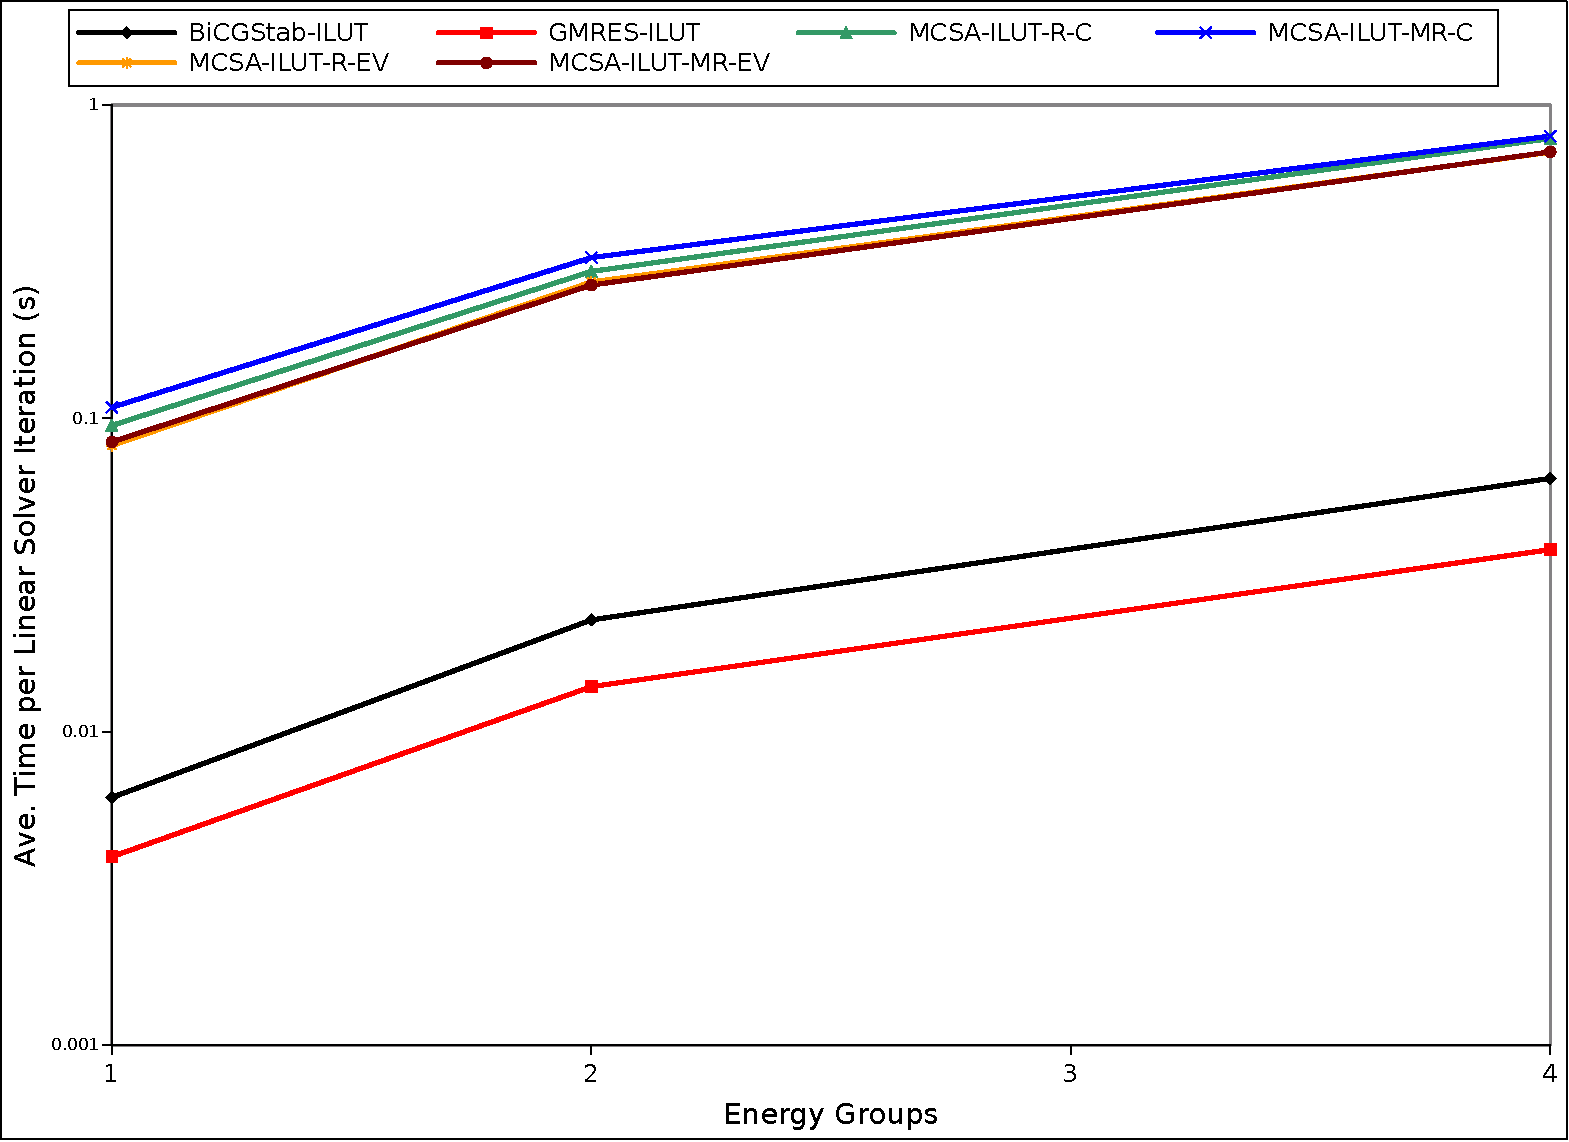
\includegraphics[width=5in]{chapters/spn_equations/solver_time.pdf}
  \end{center}
  \caption{\textbf{Average CPU time per linear solver iteration in
      seconds for the fuel assembly problem as a function of energy
      groups.}  \textit{All linear solver iterations over all
      eigenvalue iterations were used to compute the
      average. Table~\ref{tab:spn_solver_defs} gives the description
      for each solver type presented in the legend with the Krylov
      solvers represented in black and the MCSA solvers represented in
      red.}}
  \label{fig:spn_comparison_time}
\end{figure}

Finally, not considered in Figure~\ref{fig:spn_comparison_time} is the
time required to actually form the explicit inverse preconditioner
matrices and the composite operator through matrix-matrix
multiplication. The timing numbers reported were simply to perform the
MCSA iteration procedure with the composite operator already
formed. Figure~\ref{fig:spn_comparison_prec_time} additionally
presents the CPU times for MCSA convergence with the time to form the
inverse of the preconditioners and the composite linear operator
through matrix-matrix multiplication amortized over all iterations. As
is readily observed, including the costs of these operations increases
the MCSA computation time by another order of magnitude.

\begin{figure}[t!]
  \begin{center}
    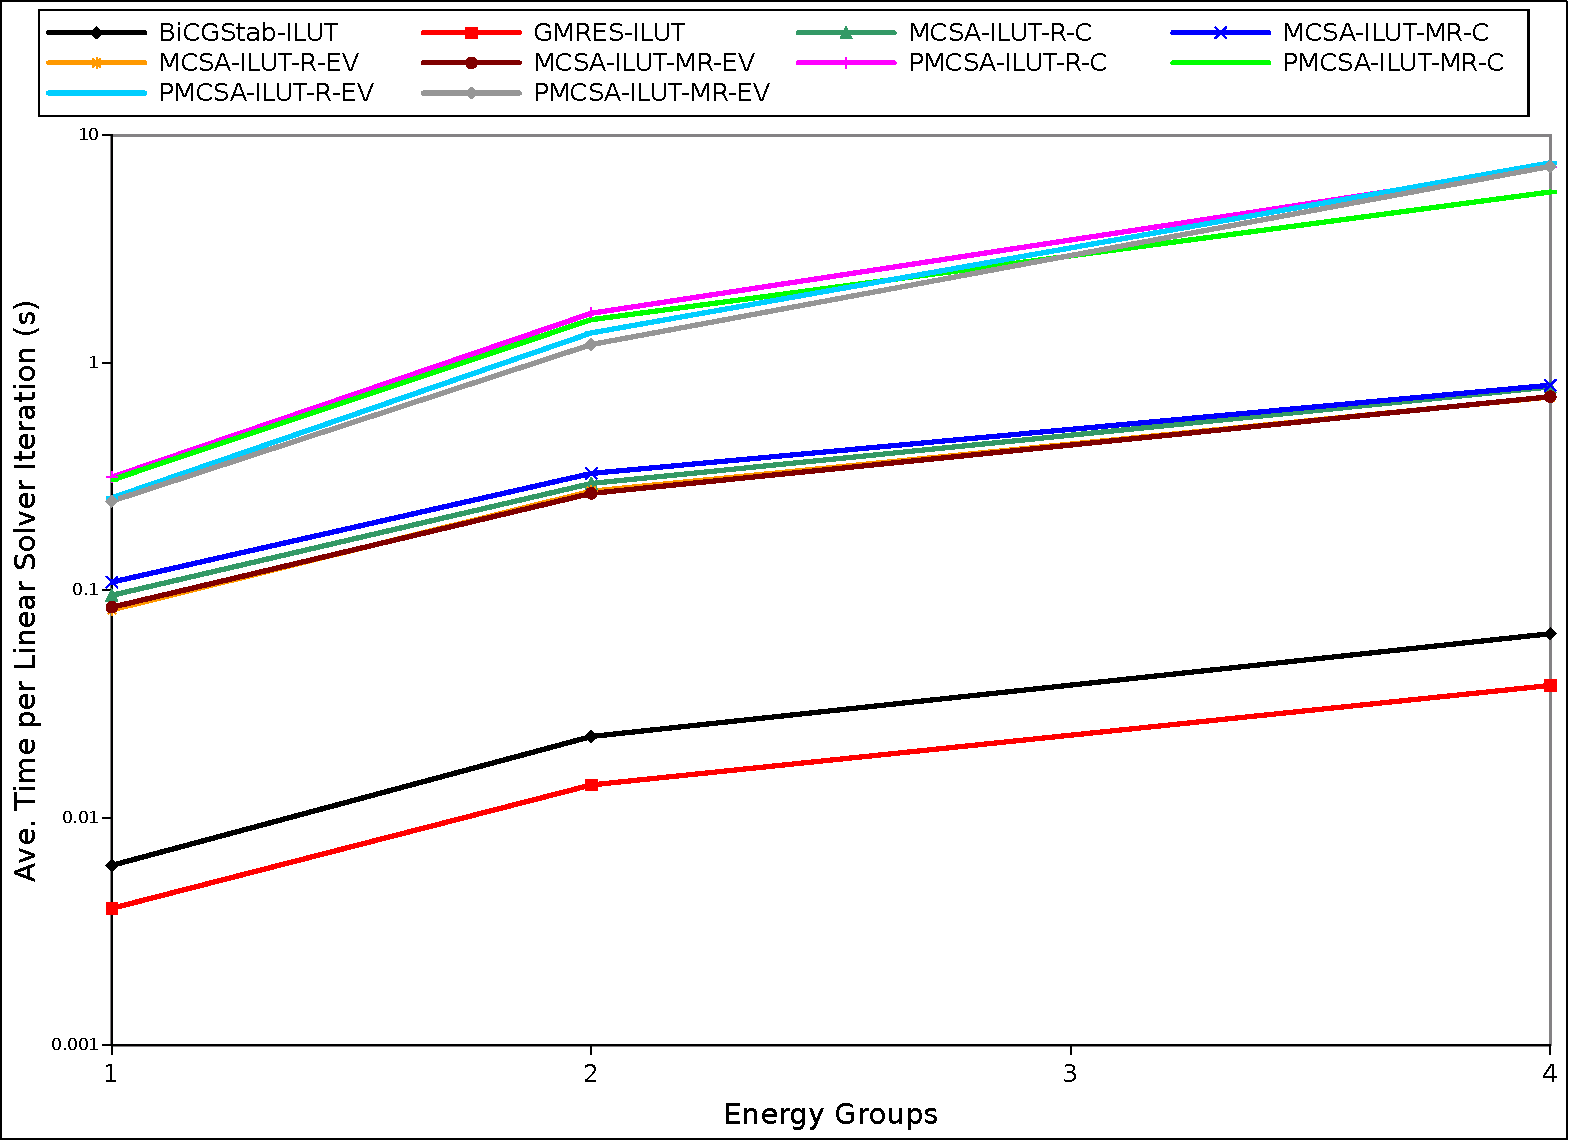
\includegraphics[width=5in]{chapters/spn_equations/solver_p_time.pdf}
  \end{center}
  \caption{\textbf{Average CPU time per iteration in seconds for the
      fuel assembly problem as a function of energy groups with
      preconditioning time included for the MCSA methods.}
    \textit{All linear solver iterations over all eigenvalue
      iterations were used to compute the
      average. Table~\ref{tab:spn_solver_defs} gives the description
      for each solver type presented in the legend. Data labeled
      starting with PMCSA and shown in blue is identical to those
      labeled with MCSA except that they additionally include the cost
      of generating the inverse of the preconditioners and composite
      linear operator.}}
  \label{fig:spn_comparison_prec_time}
\end{figure}

Based on the performance results in this section, MCSA shows promise
as a competitive and perhaps even superior method for solutions to the
neutron transport problem discretized with the $SP_N$
approximation. Not only are the correct answers produced when compared
to production linear solvers, but the iterative performance is
comparable to Krylov methods with identical preconditioning that would
typically be used every-day calculations. From a CPU timing
perspective, the methods yield the same time complexity as a function
of the number of energy groups in the problem when compared to the
Krylov methods. Here, a large time constant is generated due to the
explicit preconditioning strategy and the generation of dense linear
operators as a result. To improve these results and put general MCSA
schemes into a performance regime where they are competitive with
Krylov methods for neutron transport problems, significant research
will be required to improve upon the explicit preconditioning scheme
presented here.

\clearpage

%%---------------------------------------------------------------------------%%
\section{Summary\ }
\label{sec:mc_summary}

In this chapter, the Monte Carlo Synthetic Acceleration method has
been applied to the $SP_N$ discretization of the neutron transport
equation and explored in the context of a difficult nuclear fuel
assembly criticality problem. The following are the significant
observations and findings.

\begin{itemize}
\item MCSA can solve the asymmetric system generated by the $SP_N$
  equations
\item MCSA has been incorporated into the Exnihilo neutronics
  production code base developed at Oak Ridge National Laboratory
\item Simple Jacobi-based preconditioning reduces the spectral radius
  of the $SP_N$ system below unity, however, this alone is not
  sufficient for MCSA convergence
\item As the spectral radius approaches unity, MCSA was demonstrated
  to break down with more stochastic histories required for
  convergence and more CPU time required per history
\item Light water reactor problems are difficult to solve with MCSA as
  they have large spectral radii due to the neutron scattering in the
  moderator
\item Advanced algebraic preconditioning strategies were applied to
  the $SP_N$ equations to obtain convergence with ILUT chosen for
  subsequent investigations
\item The reduced domain approximation was required to mitigate the
  memory and performance constraints of the explicit preconditioning
  strategy although both remain significant obstacles
\item MCSA relaxation parameters were developed and observed to
  enhance the time to solution for the fuel assembly criticality
  problem
\item MCSA was verified to produce the same flux distribution and
  k-eigenvalue for the fuel assembly as production Krylov methods
\item MCSA was observed to converge in fewer iterations per eigenvalue
  iteration than GMRES for the fuel assembly criticality problem and
  more than Bi-CGStab using the same preconditioning
\item The explicit preconditioning strategy required to overcome the
  MCSA spectral radius restriction creates runtimes $O(100)$ larger
  than the production Krylov methods for the fuel assembly criticality
  problem
\end{itemize}
